\chapter[Trends]{Trends in observations and EMEP MSC-W model calculations 2000-2019}
\label{ch:Trends}

{\bf{Authors}}\\

\old{TODO}

\section{\label{sec:Trends_introduction}Introduction and background}
At its thirty-ninth session (Geneva, 9–13 December 2019), the Executive Body launched the review of the Protocol to Abate Acidification, Eutrophication and Ground-level Ozone (the Gothenburg Protocol) as amended in 2012. In order to assess  the progress made towards achieving the environmental and health objectives of the Protocol, a
list of questions was given to the subsidiary bodies of the Air Convention. Several of these questions were related to the trends of air pollution in Europe. 

In this chapter, we present an assessment of the trends in air pollution in Europe for the period 2000-2019 based on long term observational data from the EMEP network as well as EMEP MSC-W model calculations. We analyze trends in air quality for ozone, sulphur dioxide, particulate matter (and their species; sulphate, nitrate, ammonium, EC and OC) oxidized and reduced as well as wet deposition of sulphur and nitrogen species. In addition, we present trends in some indicators of health and vegetation risk (SOMO35, exceednaces of WHO guideline values for PM2.5, exceedances of critical loads for acidification and eutrophication for every 5 year since 2000).

Unfortunately, the EMEP observational network is dominated by sites in western Europe and has hardly any coverage in the EECCA & western Balkan area. 


*Domain is basically western Europe, no EECCA
*That we look from 2000 to get sign trends, not 2005

*The N-question
*That we look at OC/EC for the first time
*Chemical composition?
*Exceedances of Cls

\section{\label{EMEPmodelcalc}{Setup for EMEP MSC-W model calculations}}
The EMEP MSC-W model version rv4.42 has been used for the all the model runs for years 2000 to 2019. The horizontal resolution is \resZO, with 20 vertical layers (the lowest with a height of approximately 50 meters).
 Meteorology, emissions, boundary conditions and forest fires for the respective years have been used as input. Meteorological data have been
 derived from ECMWF-IFS(cy40r1) simulations for the years 2000 to 2018 and a ECMWF-IFS(cy46r1) simulation for 2019 (see Section~\ref{sec:meteo}). 
 The boundary conditions for the main gaseous and aerosol species were based on climatological observed values with prescribed trends in trans-Atlantic fluxes, while the Mace
Head correction has been used for ozone. The boundary conditions for natural particles of
sea salt and mineral dust were the same as in the status run, namely 5-year monthly average
concentrations, derived from EMEP MSC-W global runs, kept invariable over the calculation
period.
Daily emissions from forest fires were from the Fire INventory from NCAR (FINN) for 2002-2019,
whereas for 2000 and 2001 (unavailable from FINN), monthly averages over 2005-2015 were
used.

Volcanic \sox emissions from passive degassing of Italian volcanoes (Etna,
Stromboli and Vulcano) are those reported by
Italy. \sox and PM emissions from volcanic eruptions of Icelandic volcanoes in the period 2000-2019 (Eyjafjallaj\"okull in 2010, Gr{\'{\i}}msv{\"{o}}tn in 2011  and  Bar\dh{}arbunga in 2014-2015) are reported by Iceland. 
 
The speciation of PM emissions into OC/EC emissions was based on ECLIPSE v6b emissions. These are given in 5-year intervals (2000, 2005, etc.); intermediate years were derived by linear interpolation. However, all years after 2015 used the 2016 speciation of PM emissions.
The VOC split (speciation of NMVOC emissions) was the same as in the status run and kept constant over the period.
Soil NOX emissions were based on the new CAMS-GLOB-SOIL v2.2 NOx inventory \citet{SimpsonDarras:2021}. Soil-NOx emissions which are related to the use of fertilizer were not taken from the CAMS-GLOB-SOIL inventory, as these are already included in the EMEP (CEIP) emissions.
A revised set of anthropogenic emissions for all the years 2000-2019 has been used in the model calculations (including all the reported and re-reported data by June 2021), see chapter \ref{ch:emis2019}.

\section{\label{OBSTrends}{Observations}} NILU to write

\section{\label{Method}{Method for calculation of trends}}
Both observed and modelled trends were processed with the pyaerocom software (\url{https://github.com/metno/pyaerocom}, version XXX) for the following periods: 2000-2019, 2005-2019, 2000-2010, and 2010-2019. All observations were provided via the EBAS database. 

In order to compute trends, for each station and variable, time series data was merged in time to cover the respective time period for the trends.
Since the provided temporal resolution can change over time for a given site, the lowest common resolution was identified and higher resolution data were down-sampled to that resolution during the merging process. For temporal re-sampling, a conservative scheme was used requiring ca 75\% coverage in a hierarchical manner, that is, at least 18 hourly measurement values to retrieve a daily mean, and at least 21 daily values to retrieve a monthly mean. Trends are computed based on yearly averages, as described in more details below. To retrieve the yearly averages, at least one monthly value is required per season. In addition to trends based on yearly averages, seasonal trends are computed as well for all variables but O$_{3}$ which is focusing on the summer maximum using percentiles (details below). In addition to this conservative re-sampling scheme, a second analysis was done using 25\% coverage constraint instead of 75\% coverage. Finally, a minimum number of yearly averages was required to be available for the trends computation depending on the length of the period, corresponding to ca 75\% (e.g. 14 yearly values for the period 2000-2019).

For O$_3$, the re-sampling was done differently, that is, daily max values were computed based on hourly measurements, requiring at least 18 hourly measurements per day as for the other variables. Then, the yearly average was computed using different percentiles of the daily values (10, 50, 75, 95, 98, 99 percentiles), requiring at least 330 daily max values in a given year. Trends were then computed for each of these percentile averages.

Model output is given on daily resolution, including the daily max O$_3$. To compute the model trends, the model output for each variable was collocated in space and time with the observations. Collocation in space was done by picking the nearest model grid to each station. Collocation in time was done by first re-sampling both model and observation data to the lowest common temporal resolution, then invalidating the model output at times when observations are missing, and finally calculating the monthly mean of both. Precipitation (reported in units of mm) was collocated in time based on monthly aggregates, which were calculated independently for model and observations.

The monthly time series of the collocated model and observation data were output as csv files for each individual site. The scripts used for processing the data and calculating trends are available from a GitHub repository (\url{https://github.com/metno/emep_trends_2021}). The processed data itself, including relevant station metadata and trends results, are available in a separate location which is linked to in the description of the repository.

The same methodology as described by \cite{aas2019global, mortier2020} has been used to derive the trends at the individual stations. The significance of the trends is tested with the Mann-Kendall test \citep{hamed1998modified}. The related p-value is used to determine if the trend is significant or not within a confidence interval of 68 \%. The slope is calculated with the Theil-Sen estimator which is less sensitive to outliers than standard least-squares methods \citep{sen1968estimates}.

An uncertainty is provided for each trend by combining the error of the slope calculation itself to the error of the residuals:

\begin{equation}
 Uncertainty = \sqrt{{\left (\frac{\Delta m}{y(start)}\right )}^{2} + {\left ( \frac{m \cdot \Delta r}{y(start)^2}\right )}^{2} }
\end{equation}

where $\Delta m$ is the Theil-Sen estimator 95\% confidence interval, $y(start)$ is the value of the regression line at the first year of the period, $m$ is the value of the Theil-Sen slope and $\Delta r$ is the averaged error on the residuals computed based on the difference between the linear trend and the yearly mean values of the regional time series.

In order to allow for consistent comparisons, the trend is provided as a relative trend (\%/yr) with respect to the first year of the time period.



\section{\label{sec:Trends_sulfur}Trends in sulfur}

The SO$_x$ emissions has declined by more than 80\% in Europe the last two decades, and both the observed and modelled trends for all the atmospheric sulfur components show a substantial decrease (Figure~\ref{fig:SOx_trends} and ~\ref{tab:so2_stat} - ~\ref{tab:so4dep_stat}), in line with several studies on trends the latter years (\cite{aas2019global, Colette2012, Vivanco2018, Theobald2019, Colette2021, Banzhaf2015, torseth2012, Crippa2016}).

On average the reductions in observations for the last 20 years (2000-2019) are -3.6, -3.0 and -2.9  \% yr$^{-1}$ for \soii, \soiv in aerosols and in wet deposition respectively, while the trends in model calculations are somewhat higher: -4.9, -3.6 and -4.0 \% yr$^{-1}$, respectively. The overestimation in sulfur trends by the model is seen both for relative and absolute trends for \soii, and wet deposition of \soiv while for \soiv in aerosols the trend is higher in observations but within the confidence interval to the modelled trends. 


The  greater decrease in \soii compared to secondary sulphate is due to a combination of higher oxidation rate (hence more \soii converted to \soiv) and increased dry deposition rate of \soii. The oxidation capacity of the atmosphere have increased as the emissions have decreased \cite{Dalsoren2016}, and the clouds have become less acidic due to less \soii and only slightly decrease in \nhiii, which has increased the oxidation rate of \soii to \soiv via the ozone pathway (\cite{Banzhaf2015, Redington2009}). In addition, less acidity in the environment probably leads to more efficient dry deposition of \soii (\cite{Fowler_et_al:2009}) 




\begin{figure}
	\centering
	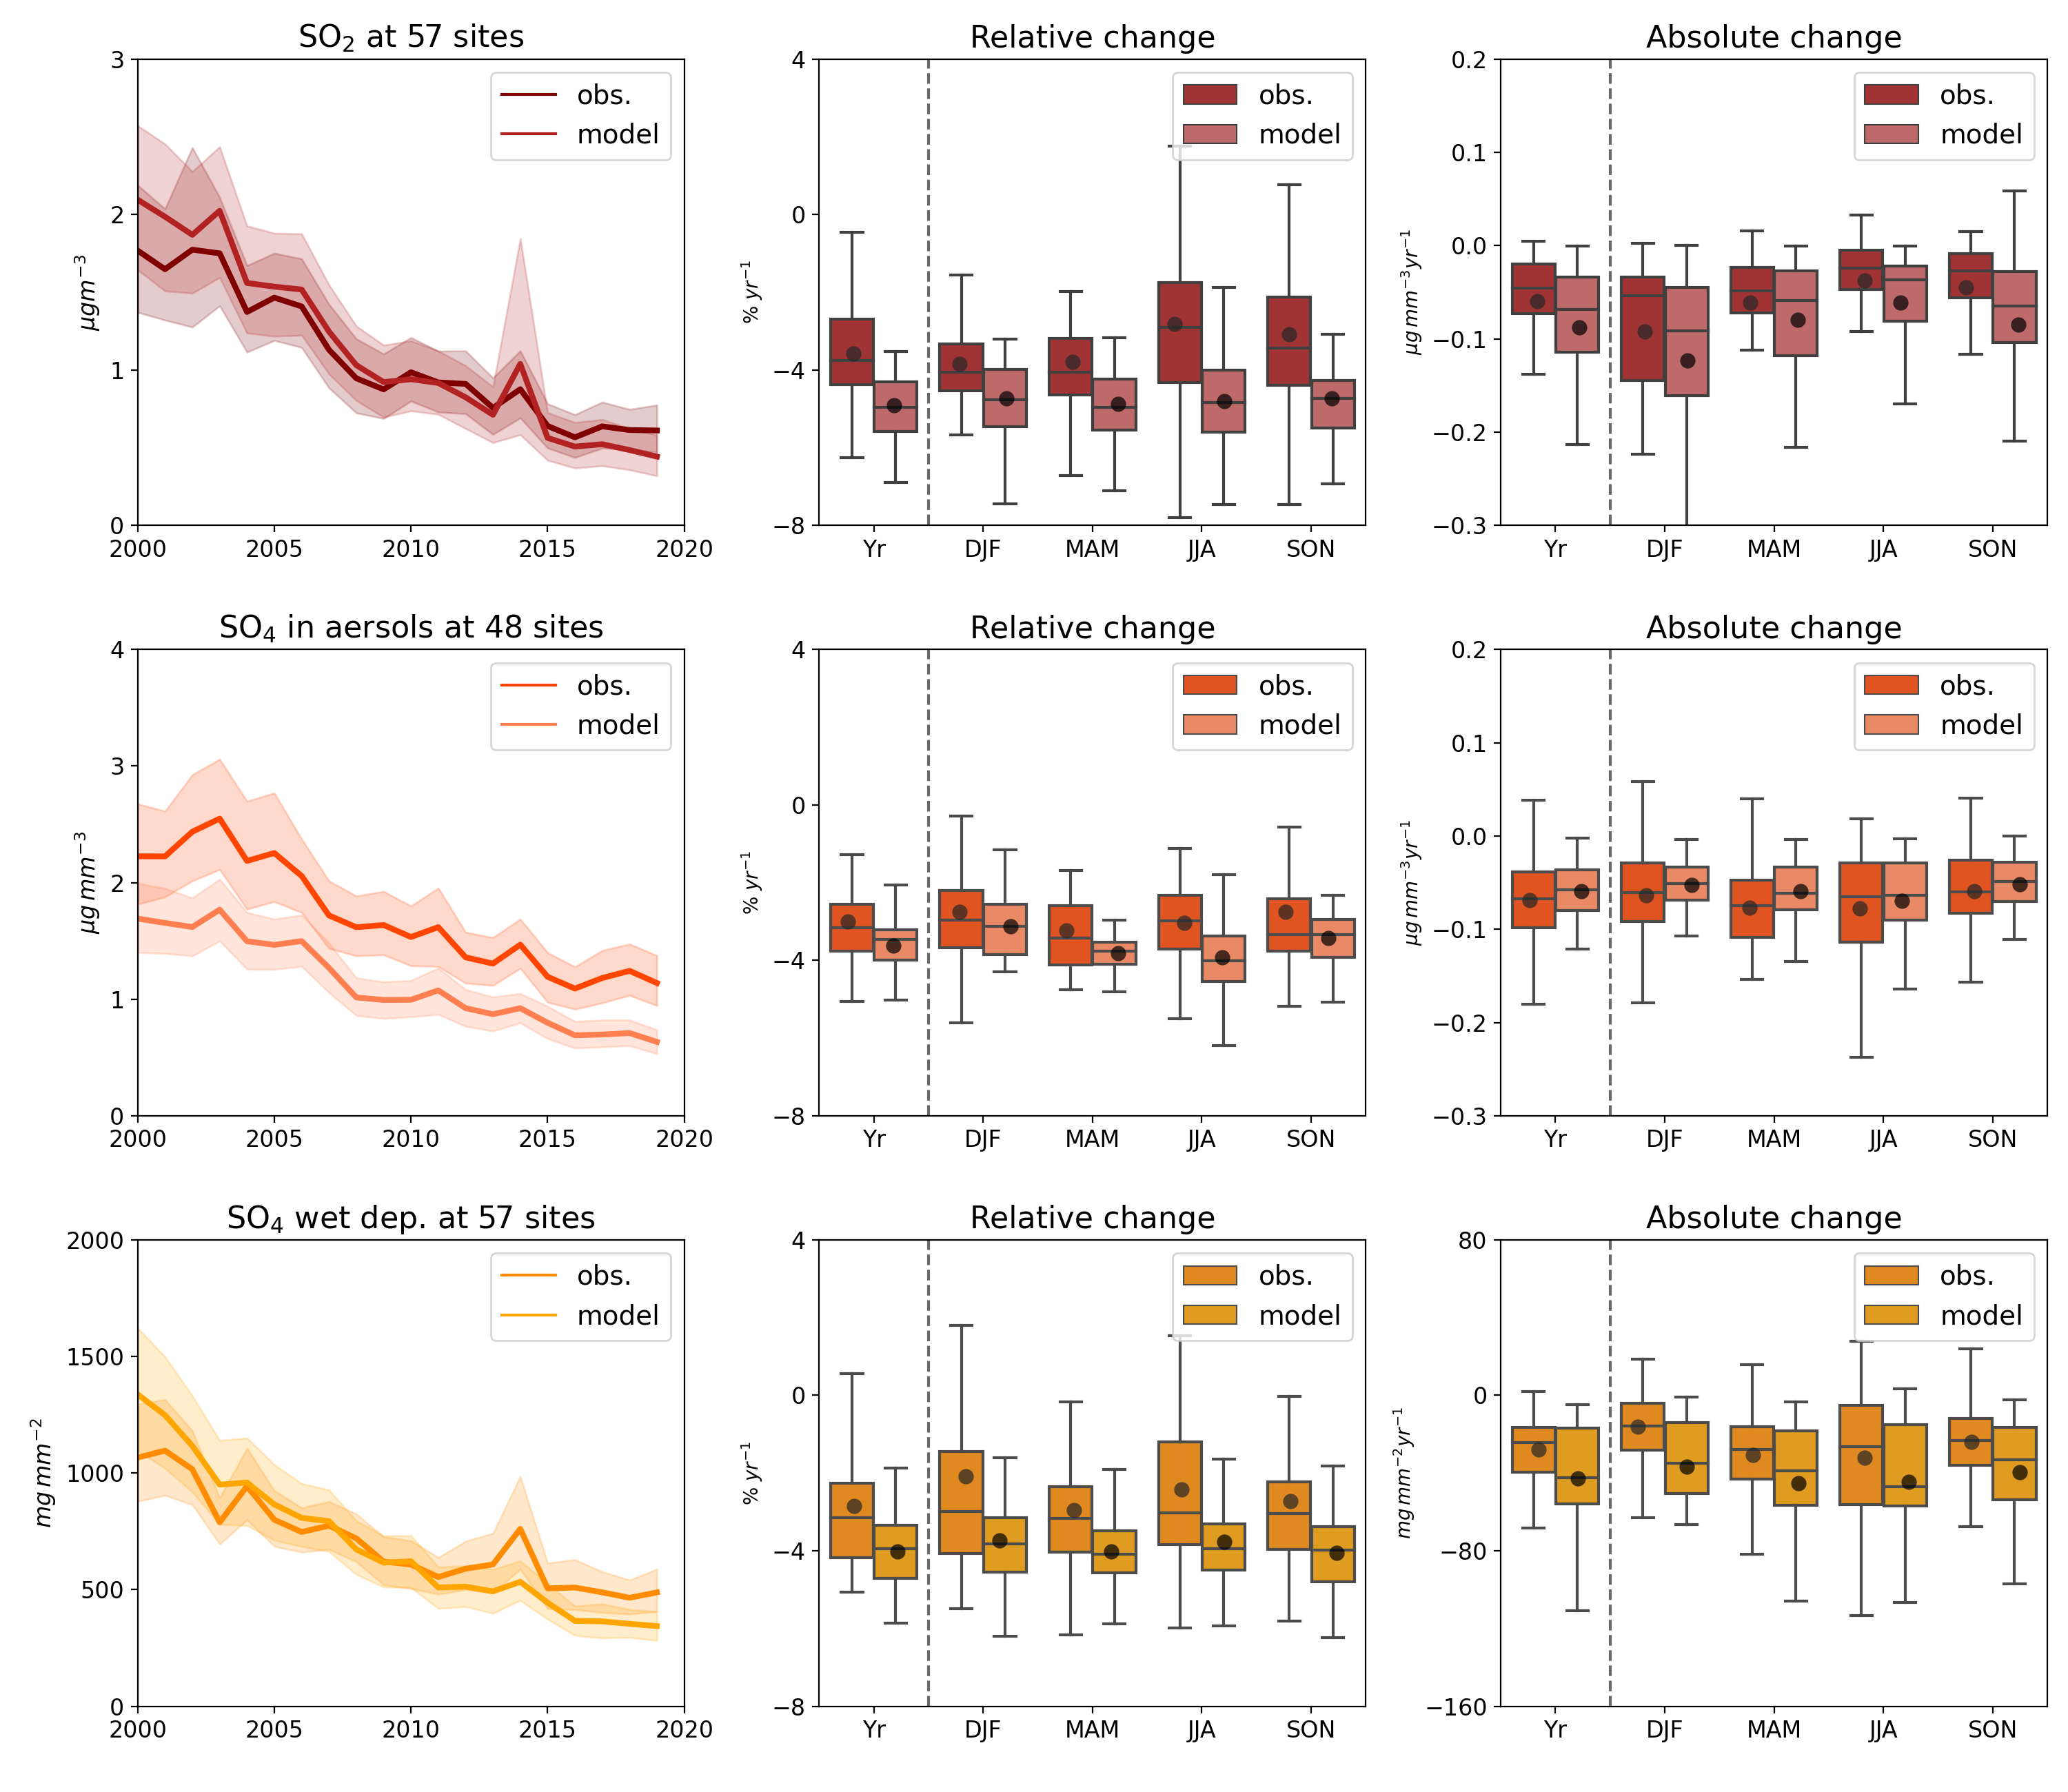
\includegraphics[width=0.74\paperwidth]{FIGS_TRENDS/sulfur_trends.png}
	\caption{\label{fig:SOx_trends}Trends in sulfur components from 2010-2019 for EMEP observations and model. The solid line in the trend plots indicate the average annual mean concentrations for all the sites and the shaded area the 95 \% confidence interval. The box plot represent the 50,25,75 percentiles and the whiskers lie within the 1.5 inter-quartile ranges for the trends of all the sites, including those with not significant trends. In addition, the mean trends are indicated with black circles}
\end{figure}

\begin{table}
\caption{\label{tab:so2_stat} Average absolute and relative changes in \soii concentrations for different periods in 2000-2019, annual and seasonal trends}
\begin{center}
\scalebox{0.65}{%
\begin{tabular}{ll|ccc|cccc|cccc}
\toprule
          &        & \multicolumn{3}{c}{Number of sites} & \multicolumn{4}{c}{Average change per year (\ug $yr^{-1})$} & \multicolumn{4}{c}{Relative change per year (\% $yr^{-1}$)} \\
Period & Seasons &           total & sign.(obs.) & sign.(mod.) &                    obs. &          conf.interval &  mod. &          conf.interval &                     obs. &         conf.interval &  mod. &        conf.interval \\
\midrule
2000-2019 & all &              48 &          46 &          48 &                  -0.068 &  (-0.085, -0.051) & -0.087 &  (-0.108, -0.067) &                    -3.88 &  (-4.23, -3.53) & -5.09 &  (-5.38, -4.79) \\
          & winter &              50 &          45 &          49 &                  -0.102 &  (-0.127, -0.076) & -0.123 &  (-0.152, -0.095) &                    -4.08 &   (-4.36, -3.8) & -4.92 &   (-5.2, -4.63) \\
          & spring &              48 &          45 &          48 &                  -0.070 &  (-0.086, -0.053) & -0.080 &     (-0.1, -0.06) &                    -4.15 &  (-4.45, -3.85) & -5.06 &   (-5.32, -4.8) \\
          & summer &              48 &          33 &          48 &                  -0.043 &  (-0.057, -0.029) & -0.060 &  (-0.078, -0.041) &                    -3.01 &  (-3.59, -2.43) & -4.93 &  (-5.29, -4.56) \\
          & autumn &              48 &          36 &          47 &                  -0.051 &  (-0.066, -0.035) & -0.085 &  (-0.106, -0.063) &                    -3.55 &  (-3.94, -3.15) & -5.00 &  (-5.28, -4.72) \\
2005-2019 & all &              57 &          41 &          53 &                  -0.055 &  (-0.068, -0.041) & -0.066 &   (-0.083, -0.05) &                    -4.27 &  (-4.72, -3.83) & -5.24 &   (-5.58, -4.9) \\
2010-2019 & all &              60 &          36 &          43 &                  -0.050 &  (-0.062, -0.037) & -0.056 &  (-0.072, -0.041) &                    -4.81 &  (-5.94, -3.69) & -6.38 &  (-7.14, -5.62) \\
2000-2010 & all &              66 &          30 &          57 &                  -0.079 &  (-0.103, -0.054) & -0.116 &  (-0.141, -0.091) &                    -3.52 &  (-4.31, -2.73) & -5.36 &  (-5.91, -4.81) \\

\bottomrule
\end{tabular}}
\end{center}
\end{table}

\begin{table}
\caption{\label{tab:so4pm_stat} Average absolute and relative changes in \soiv concentrations in aerosols for different periods in 2000-2019, annual and seasonal trends}
\begin{center}
\scalebox{0.65}{%
\begin{tabular}{ll|ccc|cccc|cccc}
\toprule
          &        & \multicolumn{3}{c}{Number of sites} & \multicolumn{4}{c}{Average change per year (\ug $yr^{-1})$} & \multicolumn{4}{c}{Relative change per year (\% $yr^{-1}$)} \\
Period & Seasons &           total & sign.(obs.) & sign.(mod.) &                    obs. &          conf.interval &  mod. &          conf.interval &                     obs. &         conf.interval &  mod. &        conf.interval \\
\midrule
2000-2019 & all &              39 &          38 &          39 &                  -0.074 &  (-0.087, -0.062) & -0.061 &   (-0.072, -0.05) &                    -3.20 &  (-3.46, -2.93) & -3.70 &  (-3.94, -3.46) \\
          & winter &              40 &          29 &          31 &                  -0.064 &   (-0.08, -0.049) & -0.055 &  (-0.065, -0.045) &                    -2.75 &  (-3.22, -2.28) & -3.15 &   (-3.39, -2.9) \\
          & spring &              38 &          36 &          38 &                  -0.085 &  (-0.098, -0.072) & -0.061 &  (-0.071, -0.051) &                    -3.46 &  (-3.72, -3.19) & -3.91 &   (-4.1, -3.72) \\
          & summer &              38 &          36 &          38 &                  -0.082 &  (-0.102, -0.063) & -0.073 &  (-0.092, -0.055) &                    -3.15 &  (-3.46, -2.85) & -4.04 &  (-4.37, -3.71) \\
          & autumn &              37 &          34 &          37 &                  -0.062 &   (-0.073, -0.05) & -0.053 &  (-0.063, -0.043) &                    -3.08 &   (-3.4, -2.76) & -3.50 &  (-3.72, -3.28) \\
2005-2019 & all &              43 &          35 &          41 &                  -0.067 &  (-0.079, -0.055) & -0.051 &   (-0.06, -0.043) &                    -3.48 &  (-3.88, -3.09) & -3.86 &   (-4.11, -3.6) \\
2010-2019 & all &              46 &          20 &          30 &                  -0.053 &  (-0.068, -0.038) & -0.043 &  (-0.054, -0.032) &                    -3.43 &  (-4.11, -2.75) & -4.22 &  (-4.89, -3.55) \\
2000-2010 & all &              54 &          15 &          41 &                  -0.068 &  (-0.085, -0.051) & -0.090 &  (-0.104, -0.075) &                    -2.51 &  (-2.95, -2.07) & -4.13 &  (-4.47, -3.79) \\
\bottomrule
\end{tabular}}
\end{center}
\end{table}

\begin{table}
\caption{\label{tab:so4dep_stat} Average absolute and relative changes in wet deposition of sulfate for different periods in 2000-2019, annual and seasonal trends}
\begin{center}
\scalebox{0.65}{%
\begin{tabular}{ll|ccc|cccc|cccc}
\toprule
          &        & \multicolumn{3}{c}{Number of sites} & \multicolumn{4}{c}{Average change per year (\ug $m^{2} yr^{-1}$)} & \multicolumn{4}{c}{Relative change per year (\% $yr^{-1}$)} \\
Period & Seasons &           total & sign.(obs.) & sign.(mod.) &                    obs. &          conf.interval &  mod. &          conf.interval &                     obs. &         conf.interval &  mod. &        conf.interval \\
\midrule
2000-2019 & all &              49 &          40 &          48 &                   -29.5 &  (-34.8, -24.2) & -43.8 &  (-52.4, -35.1) &                    -3.14 &  (-3.46, -2.82) & -4.09 &  (-4.35, -3.83) \\
          & winter &              47 &          25 &          44 &                   -19.5 &  (-24.5, -14.5) & -38.8 &  (-46.8, -30.7) &                    -2.87 &   (-3.34, -2.4) & -3.85 &  (-4.12, -3.58) \\
          & spring &              45 &          30 &          44 &                   -32.7 &  (-39.1, -26.2) & -44.8 &  (-55.1, -34.4) &                    -3.23 &   (-3.6, -2.86) & -4.03 &  (-4.28, -3.78) \\
          & summer &              47 &          31 &          43 &                   -36.5 &  (-44.5, -28.5) & -46.8 &  (-56.8, -36.8) &                    -2.95 &  (-3.35, -2.54) & -3.96 &  (-4.29, -3.62) \\
          & autumn &              46 &          27 &          42 &                   -26.7 &  (-32.3, -21.1) & -41.0 &  (-50.4, -31.5) &                    -3.00 &  (-3.49, -2.51) & -4.12 &  (-4.42, -3.82) \\
2005-2019 & all &              53 &          30 &          46 &                   -22.9 &  (-27.9, -17.9) & -32.6 &  (-38.6, -26.6) &                    -2.87 &  (-3.51, -2.22) & -4.22 &  (-4.52, -3.93) \\
2010-2019 & all &              59 &          14 &          37 &                   -20.3 &  (-26.5, -14.1) & -32.6 &  (-39.5, -25.7) &                    -2.80 &  (-3.73, -1.86) & -4.96 &  (-5.49, -4.42) \\
2000-2010 & all &              54 &          28 &          38 &                   -46.9 &  (-56.6, -37.1) & -63.0 &  (-75.9, -50.2) &                    -4.44 &  (-5.15, -3.74) & -5.20 &  (-5.62, -4.77) \\
\bottomrule
\end{tabular}}
\end{center}
\end{table}


\section{\label{sec:Trends_oxidised_nitrogen }Trends in oxidised nitrogen}



The last decades, the total emissions of NO$_x$ declined significantly in Europe, followed by declining nitrogen dioxide concentrations, total nitrate (nitric acid plus particulate nitrate) in air and oxidized nitrogen wet deposition at EMEP background sites. 
Figure~\ref{fig:NOx_trends} shows an overview of the annual and seasonal trends in oxidised nitrogen compounds from 2000 to 2019. Tables~\ref{tab:no2_stat} to \ref{tab:no3dep_stat} show absolute and relative changes in the different oxidized nitrogen compounds.

From 2000-2019, the average reductions have been on average -1.2\% yr$^{-1}$ for nitrogen dioxide concentrations at EMEP background sites (total -24\%). As NO$_2$ has a short lifetime, the trend in NO$_2$ is expected to reflect the (local) emissions of NOx. During the 2000-2019 period, NO$_x$ emissions within the western EMEP domain (EU27+UK+EFTA countries), where the dominant part of the long term EMEP observations are situated, decreased by -48\%. EMEP/MSC-W model calculations follows the reported emission reductions closely (average reductions of -2.2\% yr$^{-1}$, or in total -42\% ). 
The agreement between the trends calculated from observations and from the model (and emissions) agree well for the last period (2010-2019), with trends around -2.3\% yr$^{-1}$, whilst the trend in the first period is substantially lower in the observations than in the model calculations (and emissions). From Figure~\ref{fig:NOx_trends} it can be seen that the agreement between observations and model calculations is excellent until around 2008, but that in the year 2009 and onwards the model (and emissions) is shifted down relative to the observations. Similar results have been found in REF (Augustin/Sverres study for EEA sites versus emissions - can we refer to that?)


The trends in wet deposition of oxidized nitrogen reflects the long range transported oxidized nitrogen (NO$_x$ that has been converted to nitric acid and particulate nitrate and then washed out by rain) and is less sensitive to local changes. Also the trends for wet deposition of nitrate are lower in the observations than in the model calculations (and emissions of NOx) for the 2000-2019 period. Whilst the average trend in observations are -1.4\% yr$^{-1}$ (total of -26\%), the model calculates the trend at the same sites to be -2.1 \% yr$^{-1}$ (total of -40\%), close to the trends in emissions from the western EMEP domain (-48\%). The difference between the trend in observations (and emissions?) are largest during the first period, similar to the results for NO$_2$. However, the model overestimates nitrate wet deposition somewhat up to around 2010, and are then shifted downward and in very good agreement with observations for the years after. Note that the number of sites with significant trends for the shorter periods are small, and thus the results encumbered with more uncertainty.

For particulate nitrate, nitric acid and their sum the results are more complex. The number of sites are few (especially for nitric acid, with only 6 sites), the coverage of Europe more scattered and the quality of the measurements is worse. 

The modelled trends for 2000 to 2019 are all around -2-2.3\% per year for particulate nitrate, nitric acid and their sum - aligned with the results of NO$_2$ and wet deposition of oxidized nitrogen and the emissions. The observations show a somewhat smaller negative trend of around -1.6\% yr$^{-1}$ for the sum and around -2\% yr$^{-1}$ both for particulate nitrate and nitric acid. For the shorter periods, the number of sites with significant trends are very small, both in the model calculations and the observations, and thus the results more uncertain.
However, for all the three observations, the trend in the first period (2000-2010) is smaller than the trend in the second period, whilst the model show a rather similar trend for the sum, and larger trends in the first period for the separate components.

In summary we find that oxidized nitrogen in air and precipitation has been decreasing since 2000. However, the decrease in the observations (-24\% for NO2 and -26\% for wet deposition of oxidized nitrogen) are smaller than in model calculations (-42\% for NO2 and -40\% for wet deposition of oxidized nitrogen) and emissions (-48\% for EU27+UK+EFTA). 

\begin{figure}
	\centering
	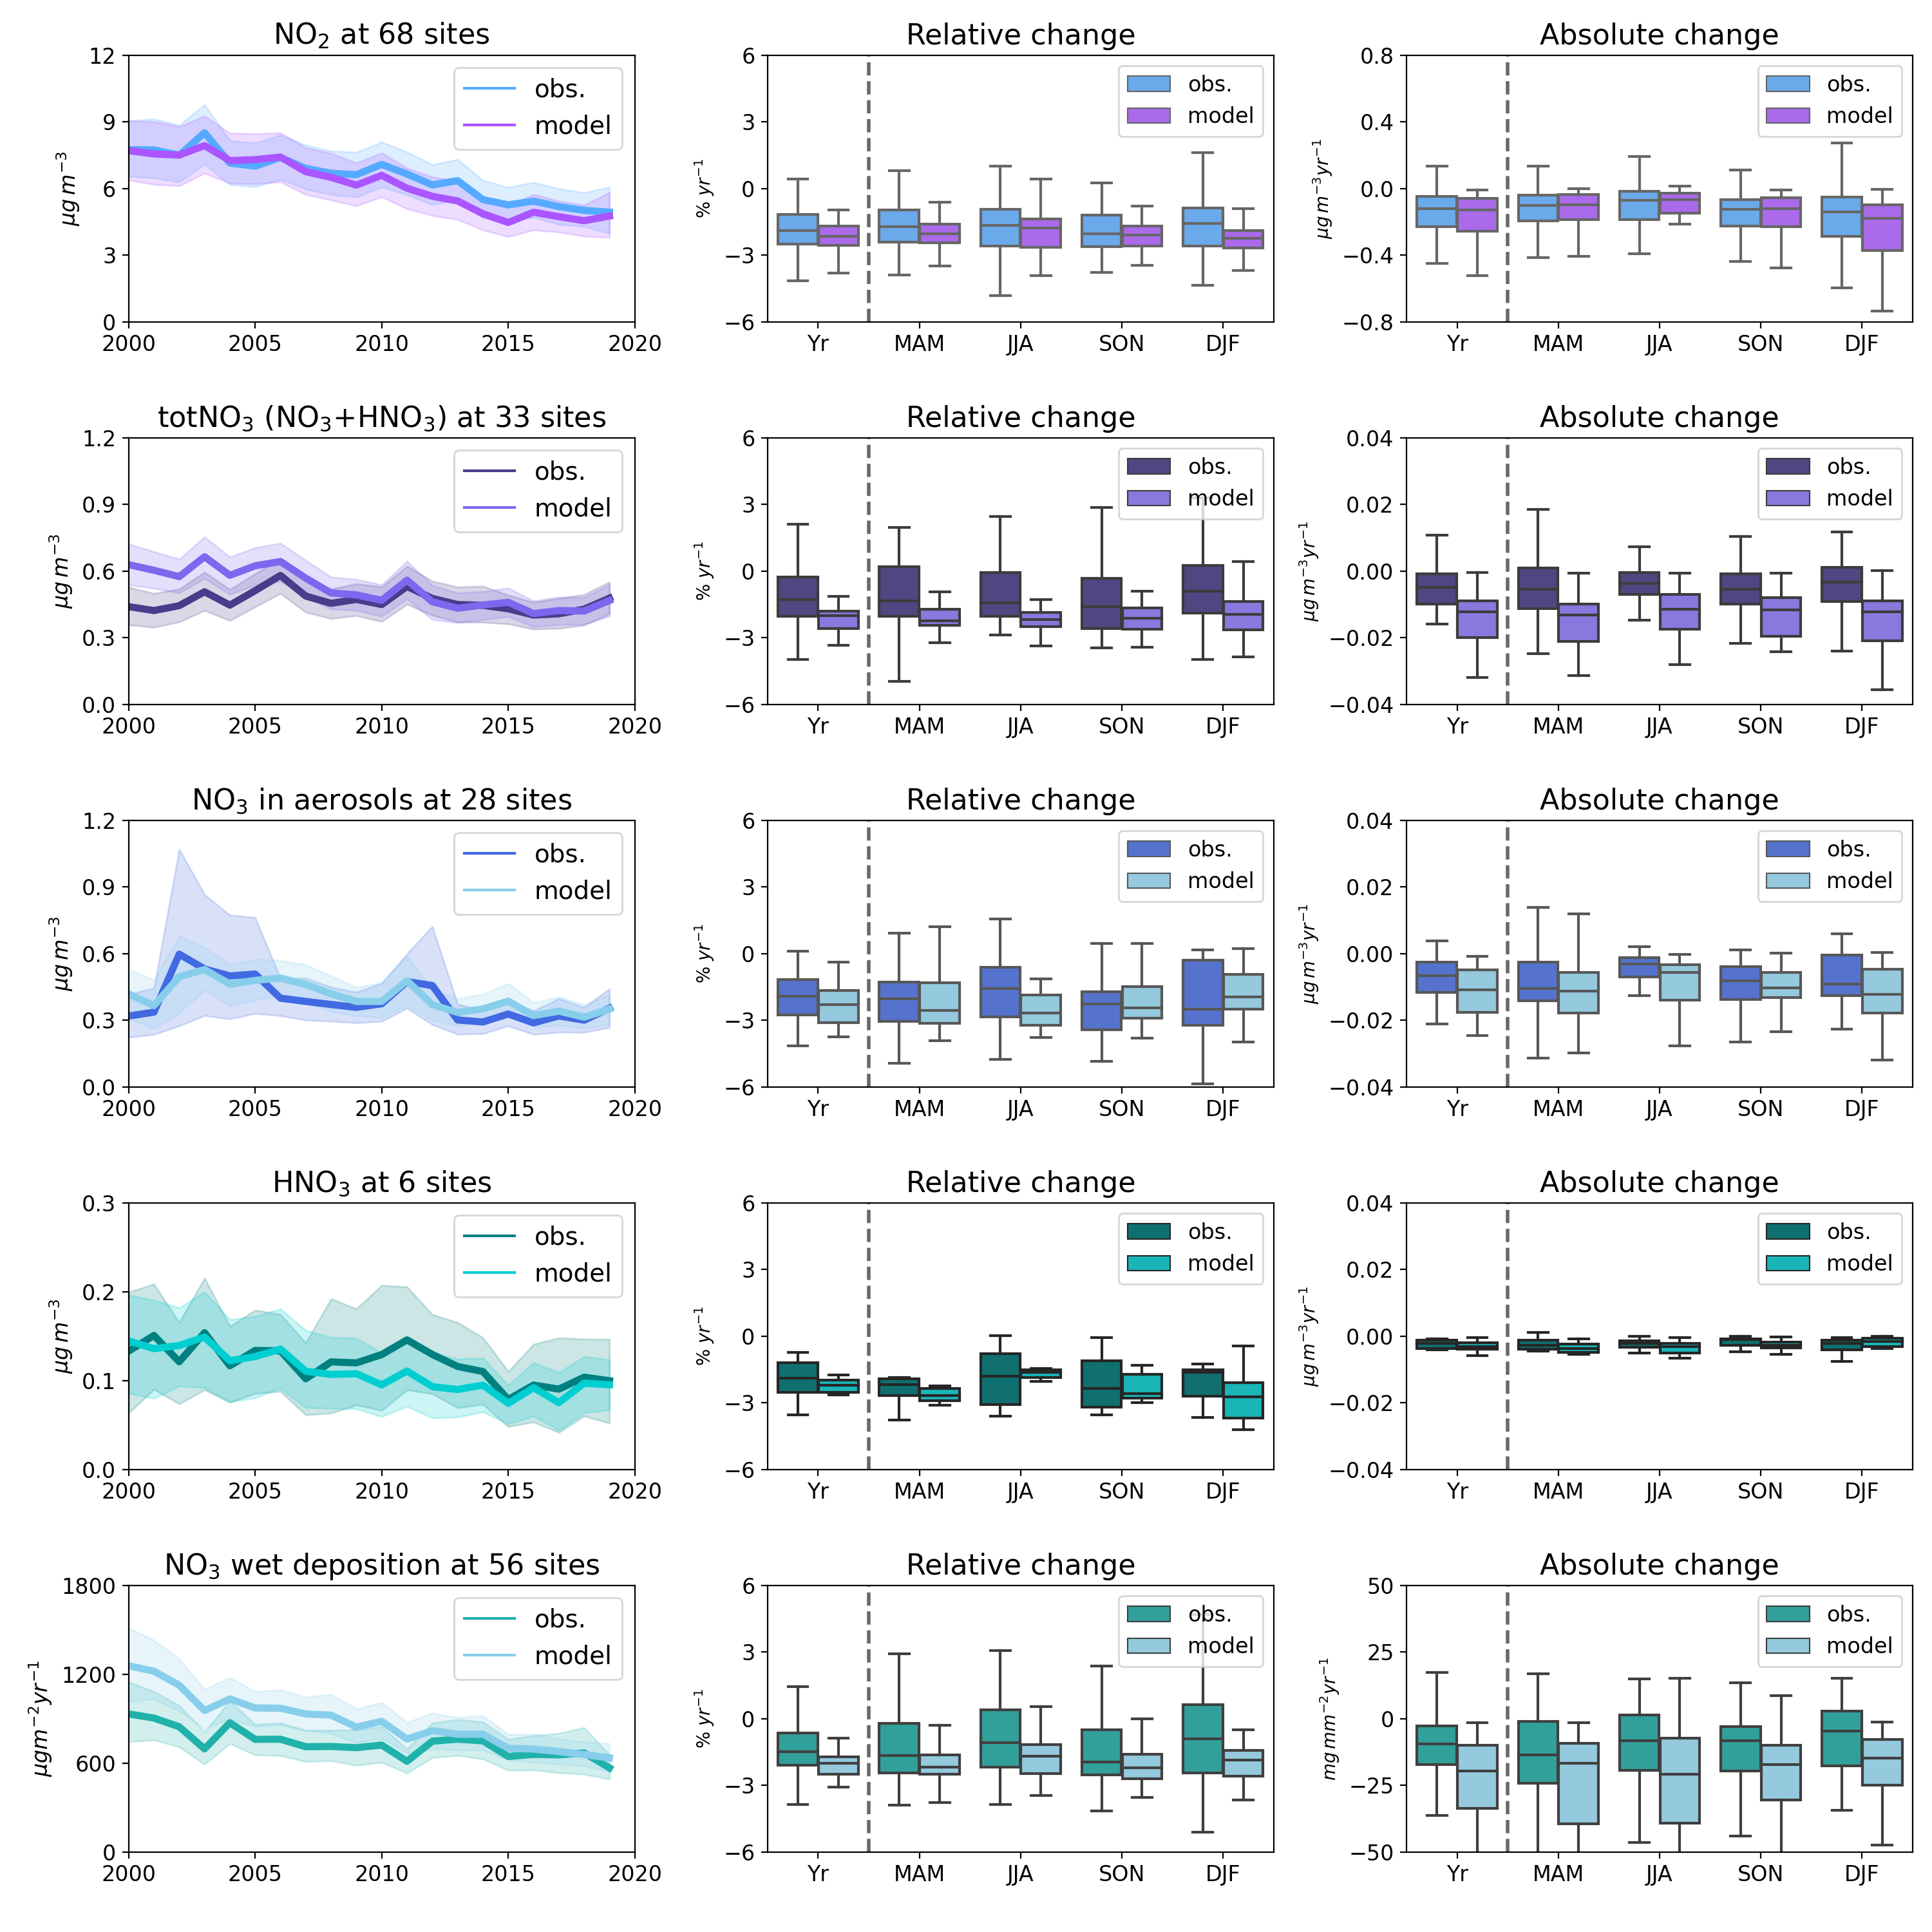
\includegraphics[width=0.74\paperwidth]{FIGS_TRENDS/Nox_trends.png}
	\caption{\label{fig:NOx_trends}Trends in oxidised nitrogen compounds from 2010-2019 for EMEP observations and model.The solid line in the trend plots indicate the average annual mean concentrations for all the sites and the shaded area the 95 \% confidence interval. The box plot represent the 50,25,75 percentiles and the whiskers lie within the 1.5 inter-quartile ranges for the trends of all the sites, including those with not significant trends. In addition, the mean trends are indicated with black circles.}
\end{figure}


\begin{table}
\caption{\label{tab:no2_stat} Absolute and relative change and corresponding confidence intervals in observed and modelled annual and seasonal aggregated \noii concentrations at the sites with 75\% data coverage  for the different time periods.The number of sites with a significant outcome is provided}
\begin{center}
\scalebox{0.65}{%
\begin{tabular}{ll|ccc|cccc|cccc}
\toprule
          &        & \multicolumn{3}{c}{Number of sites} & \multicolumn{4}{c}{Average change per year (\ug $yr^{-1})$} & \multicolumn{4}{c}{Relative change per year (\% $yr^{-1}$)} \\
Period & Seasons &           total & sign.(obs.) & sign.(mod.) &                    obs. &          conf.interval &  mod. &          conf.interval &                     obs. &         conf.interval &  mod. &        conf.interval \\
\midrule
2000-2019 & all &              59 &          44 &          58 &                  -0.132 &    (-0.164, -0.1) & -0.191 &  (-0.237, -0.146) &                    -1.16 &   (-2.2, -0.12) & -2.24 &  (-2.42, -2.06) \\
          & winter &              60 &          30 &          57 &                  -0.153 &  (-0.194, -0.112) & -0.256 &  (-0.304, -0.208) &                    -1.13 &  (-2.05, -0.21) & -2.37 &   (-2.55, -2.2) \\
          & spring &              58 &          36 &          54 &                  -0.119 &  (-0.151, -0.087) & -0.158 &  (-0.202, -0.113) &                    -0.86 &   (-2.08, 0.37) & -2.03 &  (-2.23, -1.83) \\
          & summer &              58 &          38 &          54 &                  -0.092 &  (-0.118, -0.067) & -0.134 &  (-0.177, -0.091) &                    -1.15 &  (-2.05, -0.25) & -1.88 &  (-2.13, -1.63) \\
          & autumn &              58 &          40 &          57 &                  -0.150 &  (-0.187, -0.112) & -0.191 &  (-0.239, -0.143) &                    -1.12 &   (-2.41, 0.18) & -2.19 &  (-2.38, -2.01) \\
2005-2019 & all &              63 &          48 &          62 &                  -0.161 &  (-0.196, -0.126) & -0.195 &  (-0.239, -0.151) &                    -1.84 &  (-2.55, -1.13) & -2.57 &  (-2.79, -2.35) \\
2010-2019 & all &              66 &          35 &          49 &                  -0.182 &   (-0.225, -0.14) & -0.166 &  (-0.205, -0.127) &                    -2.61 &  (-3.34, -1.88) & -2.46 &  (-2.74, -2.18) \\
2000-2010 & all &              63 &          11 &          40 &                  -0.094 &  (-0.143, -0.045) & -0.179 &  (-0.231, -0.128) &                    -1.01 &  (-1.76, -0.26) & -1.93 &   (-2.3, -1.56) \\
\bottomrule
\end{tabular}}
\end{center}
\end{table}


\begin{table}
\caption{\label{tab:tno3_stat} Average absolute and relative changes in  concentration of total nitrate ({\ensuremath{\mbox{HNO}_{\rm 3}}} + \noiii) in air and aerosols}
\begin{center}
\scalebox{0.65}{%
\begin{tabular}{ll|ccc|cccc|cccc}
\toprule
          &        & \multicolumn{3}{c}{Number of sites} & \multicolumn{4}{c}{Average change per year (\ug $yr^{-1})$} & \multicolumn{4}{c}{Relative change per year (\% $yr^{-1}$)} \\
Period & Seasons &           total & sign.(obs.) & sign.(mod.) &                    obs. &          conf.interval &  mod. &          conf.interval &                     obs. &         conf.interval &  mod. &        conf.interval \\
\midrule
2000-2019 & all &              25 &          17 &          24 &                  -0.008 &  (-0.011, -0.005) & -0.013 &   (-0.016, -0.01) &                    -1.60 &    (-2.0, -1.2) & -2.01 &   (-2.2, -1.81) \\
          & winter &              27 &           7 &          16 &                  -0.009 &  (-0.014, -0.003) & -0.015 &   (-0.019, -0.01) &                    -1.21 &  (-1.75, -0.66) & -1.89 &  (-2.22, -1.56) \\
          & spring &              25 &          13 &          21 &                  -0.010 &  (-0.013, -0.007) & -0.014 &   (-0.017, -0.01) &                    -1.69 &  (-2.08, -1.29) & -1.97 &  (-2.21, -1.73) \\
          & summer &              25 &          17 &          21 &                  -0.005 &  (-0.007, -0.003) & -0.011 &  (-0.014, -0.008) &                    -1.43 &   (-1.86, -1.0) & -2.02 &  (-2.21, -1.83) \\
          & autumn &              24 &          16 &          14 &                  -0.009 &  (-0.013, -0.006) & -0.014 &   (-0.018, -0.01) &                    -1.89 &  (-2.43, -1.35) & -2.10 &  (-2.37, -1.83) \\
2005-2019 & all &              31 &          18 &          25 &                  -0.011 &  (-0.014, -0.008) & -0.014 &  (-0.017, -0.011) &                    -2.29 &  (-2.74, -1.84) & -2.34 &  (-2.62, -2.05) \\
2010-2019 & all &              29 &          16 &           6 &                  -0.015 &   (-0.019, -0.01) & -0.010 &  (-0.014, -0.007) &                    -3.38 &   (-4.26, -2.5) & -1.99 &   (-2.4, -1.57) \\
2000-2010 & all &              32 &           7 &          12 &                  -0.006 &  (-0.011, -0.001) & -0.017 &  (-0.022, -0.012) &                    -0.56 &    (-1.6, 0.48) & -2.03 &  (-2.67, -1.39) \\
\bottomrule
\end{tabular}}
\end{center}
\end{table}

\begin{table}
\caption{\label{tab:no3pm_stat} Average absolute and relative changes in \noiii concentrations in aerosols}
\begin{center}
\scalebox{0.65}{%
\begin{tabular}{ll|ccc|cccc|cccc}
\toprule
          &        & \multicolumn{3}{c}{Number of sites} & \multicolumn{4}{c}{Average change per year (\ug $yr^{-1})$} & \multicolumn{4}{c}{Relative change per year (\% $yr^{-1}$)} \\
Period & Seasons &           total & sign.(obs.) & sign.(mod.) &                    obs. &          conf.interval &  mod. &          conf.interval &                     obs. &         conf.interval &  mod. &        conf.interval \\
\midrule
2000-2019 & all &              21 &          13 &          15 &                  -0.009 &  (-0.012, -0.006) & -0.013 &  (-0.018, -0.008) &                    -2.01 &  (-2.49, -1.53) & -2.33 &   (-2.65, -2.0) \\
          & winter &              20 &           8 &           5 &                  -0.012 &  (-0.018, -0.005) & -0.012 &  (-0.016, -0.008) &                    -1.85 &  (-2.77, -0.93) & -1.83 &  (-2.54, -1.12) \\
          & spring &              20 &          12 &          14 &                  -0.011 &  (-0.017, -0.005) & -0.012 &  (-0.017, -0.006) &                    -1.89 &  (-2.69, -1.09) & -1.93 &  (-2.74, -1.12) \\
          & summer &              20 &           8 &          12 &                  -0.004 &  (-0.006, -0.002) & -0.009 &  (-0.013, -0.006) &                    -1.55 &  (-2.17, -0.94) & -2.39 &  (-2.72, -2.06) \\
          & autumn &              20 &          11 &           8 &                  -0.010 &  (-0.013, -0.007) & -0.013 &   (-0.02, -0.007) &                    -2.41 &   (-2.8, -2.01) & -2.24 &   (-2.7, -1.78) \\
2005-2019 & all &              26 &          11 &          16 &                  -0.011 &  (-0.015, -0.006) & -0.013 &  (-0.018, -0.009) &                    -2.32 &  (-2.84, -1.81) & -2.54 &  (-2.95, -2.13) \\
2010-2019 & all &              32 &           3 &           5 &                  -0.010 &  (-0.015, -0.004) & -0.009 &  (-0.013, -0.004) &                    -1.98 &  (-2.85, -1.11) & -1.33 &  (-2.14, -0.52) \\
2000-2010 & all &              20 &           3 &           9 &                  -0.006 &   (-0.013, 0.001) & -0.019 &  (-0.027, -0.011) &                    -1.54 &   (-2.8, -0.27) & -2.81 &  (-3.82, -1.79) \\
\bottomrule
\end{tabular}}
\end{center}
\end{table}

\begin{table}
\caption{\label{tab:hno3_stat} Average absolute and relative changes in {\ensuremath{\mbox{HNO}_{\rm 3}}} concentrations}
\begin{center}
\scalebox{0.65}{%
\begin{tabular}{ll|ccc|cccc|cccc}
\toprule
          &        & \multicolumn{3}{c}{Number of sites} & \multicolumn{4}{c}{Average change per year (\ug $yr^{-1})$} & \multicolumn{4}{c}{Relative change per year (\% $yr^{-1}$)} \\
Period & Seasons &           total & sign.(obs.) & sign.(mod.) &                    obs. &          conf.interval &  mod. &          conf.interval &                     obs. &         conf.interval &  mod. &        conf.interval \\
\midrule
2000-2019 & all &               6 &           4 &           6 &                  -0.002 &  (-0.004, -0.001) & -0.003 &  (-0.005, -0.002) &                    -1.94 &  (-2.77, -1.11) & -2.24 &  (-2.53, -1.95) \\
          & winter &               6 &           3 &           4 &                  -0.003 &  (-0.005, -0.001) & -0.002 &  (-0.003, -0.001) &                    -2.15 &  (-2.92, -1.37) & -2.76 &  (-3.73, -1.79) \\
          & spring &               6 &           4 &           5 &                  -0.002 &  (-0.004, -0.001) & -0.003 &  (-0.005, -0.002) &                    -2.05 &  (-3.15, -0.95) & -2.47 &   (-2.95, -2.0) \\
          & summer &               6 &           3 &           5 &                  -0.002 &  (-0.004, -0.001) & -0.004 &  (-0.005, -0.002) &                    -1.83 &   (-2.97, -0.7) & -1.67 &  (-1.87, -1.47) \\
          & autumn &               6 &           3 &           6 &                  -0.002 &    (-0.003, -0.0) & -0.003 &  (-0.004, -0.001) &                    -2.09 &  (-3.22, -0.97) & -2.36 &  (-2.87, -1.85) \\
2005-2019 & all &              12 &           7 &           9 &                  -0.004 &  (-0.005, -0.003) & -0.002 &  (-0.004, -0.001) &                    -2.48 &   (-3.16, -1.8) & -2.01 &   (-2.63, -1.4) \\
2010-2019 & all &              16 &           4 &           1 &                  -0.005 &  (-0.007, -0.003) & -0.002 &    (-0.003, -0.0) &                    -4.25 &  (-5.65, -2.86) & -0.58 &   (-2.23, 1.08) \\
2000-2010 & all &              10 &           3 &           4 &                  -0.006 &     (-0.012, 0.0) & -0.005 &  (-0.007, -0.003) &                    -1.63 &   (-3.86, 0.61) & -3.30 &  (-4.17, -2.44) \\
\bottomrule
\end{tabular}}
\end{center}
\end{table}


\begin{table}
\caption{\label{tab:no3dep_stat} Average absolute and relative changes in wet deposition of nitrate}
\begin{center}
\scalebox{0.7}{%
\begin{tabular}{ll|ccc|cccc|cccc}
\toprule
          &        & \multicolumn{3}{c}{Number of sites} & \multicolumn{4}{c}{Average change per year (\ugN $m^{2} yr^{-1}$)} & \multicolumn{4}{c}{Relative change per year (\% $yr^{-1}$)} \\
Period & Seasons &           total & sign.(obs.) & sign.(mod.) &                    obs. &          conf.interval &  mod. &          conf.interval &                     obs. &         conf.interval &  mod. &        conf.interval \\
\midrule
2000-2019 & all &              46 &          21 &          41 &                   -12.1 &   (-15.7, -8.5) & -24.3 &  (-29.3, -19.4) &                    -1.36 &    (-1.74, -0.98) & -2.08 &  (-2.22, -1.94) \\
          & winter &              45 &           6 &          24 &                    -8.3 &   (-12.4, -4.3) & -19.1 &  (-22.8, -15.5) &                    -1.16 &    (-1.69, -0.63) & -2.08 &  (-2.31, -1.85) \\
          & spring &              43 &          17 &          30 &                   -14.2 &   (-20.5, -7.9) & -26.0 &  (-33.4, -18.5) &                    -1.11 &    (-1.74, -0.48) & -2.01 &  (-2.24, -1.78) \\
          & summer &              45 &          10 &          28 &                   -11.3 &   (-16.3, -6.2) & -27.4 &  (-34.3, -20.6) &                    -0.02 &     (-1.83, 1.78) & -1.86 &  (-2.15, -1.57) \\
          & autumn &              45 &          12 &          23 &                   -12.8 &   (-16.6, -9.0) & -23.6 &  (-29.4, -17.7) &                    -1.53 &    (-2.01, -1.05) & -2.08 &  (-2.32, -1.84) \\
2005-2019 & all &              50 &          15 &          35 &                   -10.0 &   (-14.8, -5.2) & -22.1 &  (-25.7, -18.5) &                    -0.53 &     (-2.04, 0.98) & -2.30 &  (-2.48, -2.12) \\
2010-2019 & all &              57 &           6 &          16 &                   -12.6 &   (-16.8, -8.4) & -21.8 &  (-26.5, -17.0) &                    -1.50 &    (-2.19, -0.81) & -2.22 &  (-2.66, -1.79) \\
2000-2010 & all &              45 &           8 &          13 &                   -13.2 &   (-20.8, -5.5) & -24.5 &  (-32.5, -16.5) &                    -1.12 &    (-2.22, -0.03) & -2.00 &  (-2.41, -1.59) \\
\bottomrule
\end{tabular}}
\end{center}
\end{table}



\section{\label{sec:Trends_reduced nitrogen }Trends in reduced nitrogen}
Ammonia emissions from agricultural activities have been only slightly reduced for the western EMEP domain since 2000 (-12\% in EU27+UK+EFTA countries). In the EMEP domain as a whole, ammonia emissions have increased by 12\% since 2000 (see chapter XXX).

With such small changes in emissions, clearly it is very difficult to detect any trends in the observations - considering also that the meteorological variability introduces year to year changes of the same magnitude as the expected trends.

Figure~\ref{fig:Nred_trends} shows an overview of the annual and seasonal trends in reduced nitrogen compounds from 2000 to 2019. Tables~\ref{tab:tnh4_stat} to \ref{tab:nh4dep_stat} show absolute and relative changes in the different reduced nitrogen compounds.

Indeed, both observations and model calculations find very few significant trends in wet deposition of reduced nitrogen. Out of 47 sites with long term measurements at EMEP background sites, only 14 (8) are significant for the observations (model). The average change in the observations for 2000 to 2019 is -0.14\% yr$^{-1}$, with a confidence interval from -0.1\% yr$^{-1}$ to +0.52\% yr$^{-1}$, while the model show an average trend of -0.4\% yr$^{-1}$ and a confidence interval of -0.7\% yr$^{-1}$ to -0.1\% yr$^{-1}$. For the shorter time periods (2000-2010 and 2010-2019) there are even fewer sites with significant trends (see Table~\ref{tab:nh4dep_stat}).

Total ammonium (NH$_3$ + NH$_4$)) in air show a more negative trend in observations (and model calculations) of about -1.45\% yr$^{-1}$ (-1.33\% yr$^{-1}$) and with a larger fraction of the sites having significant trends. This trends is larger than the reduction in ammonia emissions for EU27+UK+EFTA countries (-12\%), in total 27\% (25\%) in observations and model calculations for 2000-2019.

The trend for ammonium aerosols is even more negative, -2.61 and -2.51 \% yr$^{-1}$ in observations and model calculations, respectively.

Very few sites have long term time series of ammonia in air (8 sites), and very few of the trends calculated are significant. However, on average, the trends observed and calculated are positive: +1.55 and +1.28 \% yr$^{-1}$ in observations and model calculations, respectively, with all values within the confidence interval being positive.

This large difference between the trends of the different reduced nitrogen components can be explained by the interaction of ammonia with the sulphur and nitrogen components. When ammonia is released into the air, it reacts with secondary sulphate originating from the SO$_x$ emissions and forms particulate ammonium sulphates. If more ammonia is available, it reacts with nitric acid in an equilibrium reaction to form particulate ammonium nitrate. During the years from 2000 onwards, large reductions in SO$_x$ and NO$_x$ emissions have taken place, and thus less sulphate and nitric acid is available for forming ammonium particles. Therefore, a smaller fraction of NH$_3$ is converted to aerosol ammonium, and the decrease in particulate ammonium is strongly linked to the decrease in sulphate and nitrate. It is therefore to be expected that the trend in ammonium aerosol (-2.6\% yr$^{-1}$, observations) lies somewhere between the trend in particulate sulphate (-3.21, observations) and nitrate -2.01\% yr$^{-1}$). 

When less ammonia is converted to ammonium, the (very small) decrease in ammonia emissions is compensated by a larger part of ammonia residing in gas phase, and no decrease in ammonia (very few significant trends) are detected.

For the sum of ammonia and ammonium, the two opposite trends of ammonia (no trend or slighly positive) and ammonium (negative) results in a negative trend that is smaller than the trend for ammonium alone.

The analysis done for the shorter time periods (2000-2010 and 2010-2019) confirms the findings discussed above. It is worth to note that the agreement between the trends calculated from model calculations and the observation are excellent for the different reduced nitrogen components, which indicates that the EMEP MSC-W model does a very good job in reproducing the non-linear interactions between sulphur, oxidized nitrogen and reduced nitrogen and how it has evolved during the past 20 years.

In summary, the observations and the model calculations confirms that very small reductions of ammonia emissions have been achieved during the 2000-2019 period. However, the contribution of ammonia emission to aerosols have been largely reduced during this period, due to the impact of SO$_x$ and NO$_x$ emission reductions.





\begin{figure}
	\centering
	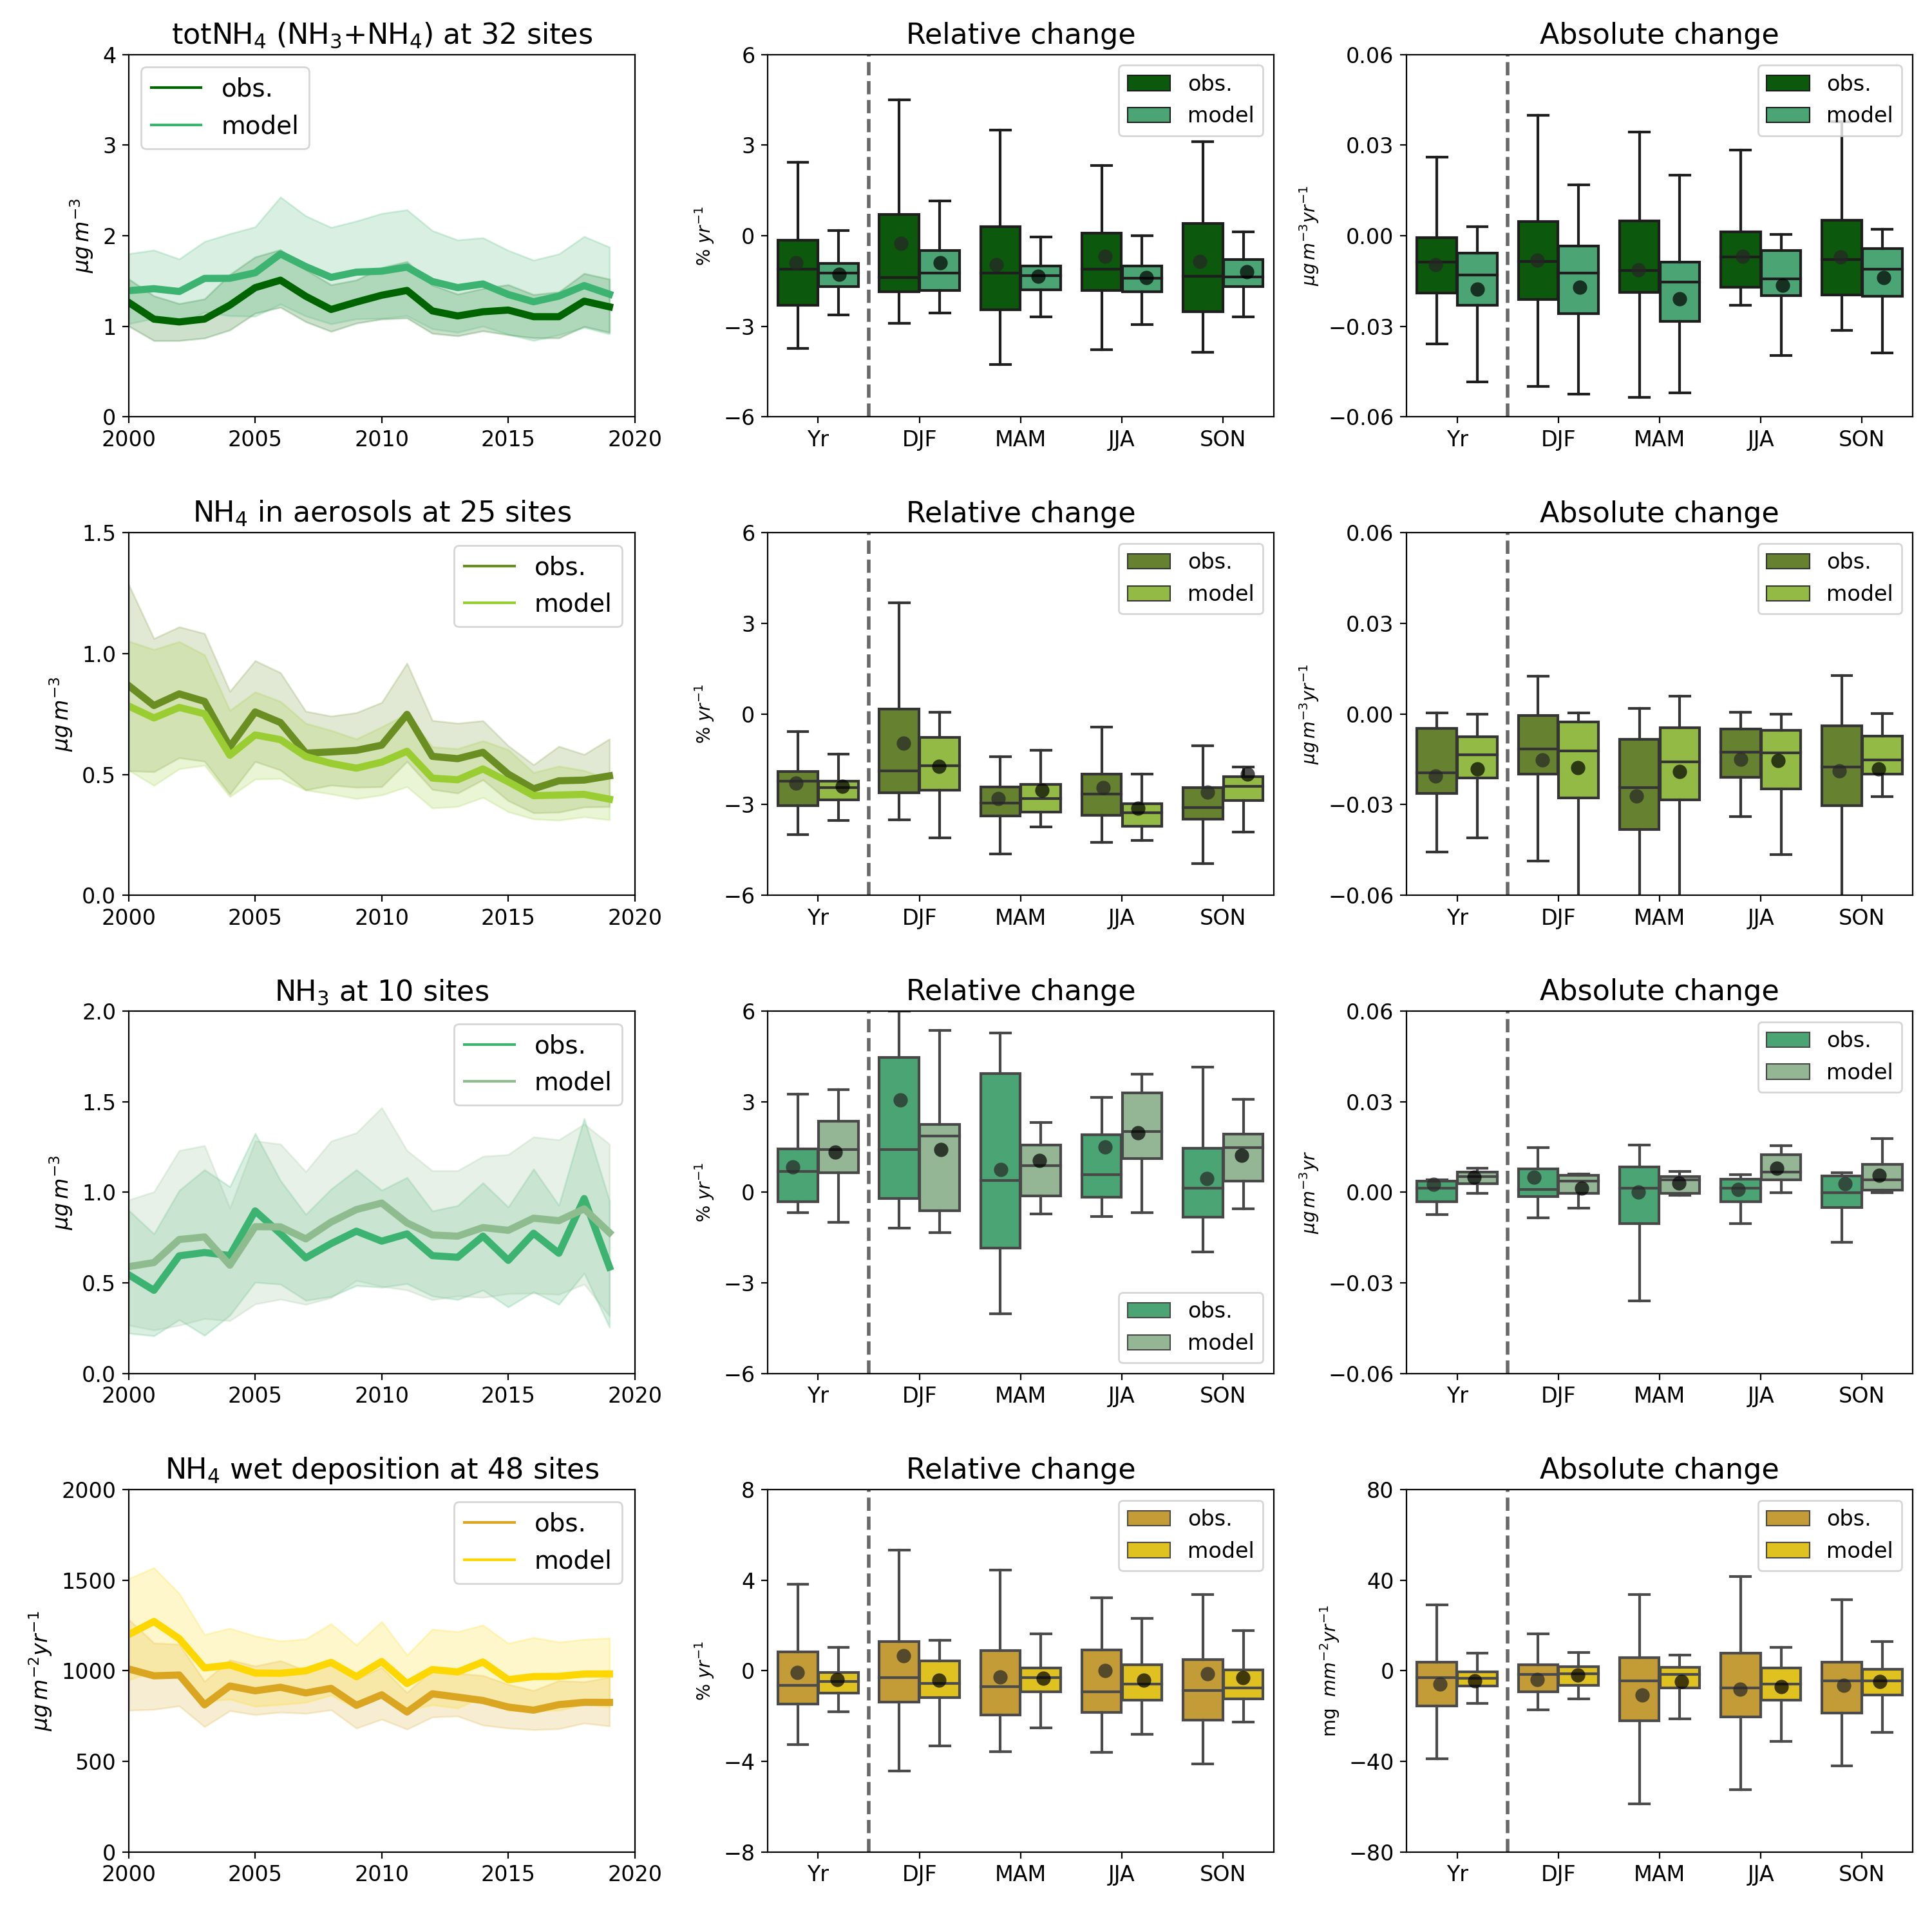
\includegraphics[width=0.74\paperwidth]{FIGS_TRENDS/Nred_trends.png}
	\caption{\label{fig:Nred_trends}Trends in oxidised nitrogen components from 2010-2019 for EMEP observations and model.The solid line in the trend plots indicate the average annual mean concentrations for all the sites and the shaded area the 95 \% confidence interval. The box plot represent the 50,25,75 percentiles and the whiskers lie within the 1.5 inter-quartile ranges for the trends of all the sites, including those with not significant trends. In addition, the mean trends are indicated with black circles.}
\end{figure}



\begin{table}
\caption{\label{tab:tnh4_stat} Average absolute and relative changes in  concentration of total ammonium (\nhiii+\nhiv) in air and aerosols}
\begin{center}
\scalebox{0.65}{%
\begin{tabular}{ll|ccc|cccc|cccc}
\toprule
          &        & \multicolumn{3}{c}{Number of sites} & \multicolumn{4}{c}{Average change per year (\ug $yr^{-1})$} & \multicolumn{4}{c}{Relative change per year (\% $yr^{-1}$)} \\
Period & Seasons &           total & sign.(obs.) & sign.(mod.) &                    obs. &          conf.interval &  mod. &          conf.interval &                     obs. &         conf.interval &  mod. &        conf.interval \\
\midrule
2000-2019 & all &              25 &          17 &          17 &                  -0.016 &  (-0.024, -0.007) & -0.019 &  (-0.027, -0.012) &                    -1.45 &  (-1.99, -0.91) & -1.33 &  (-1.54, -1.11) \\
          & winter &              28 &           9 &          10 &                  -0.018 &  (-0.029, -0.008) & -0.023 &  (-0.033, -0.013) &                    -1.18 &  (-1.72, -0.64) & -1.13 &   (-1.46, -0.8) \\
          & spring &              25 &          10 &          16 &                  -0.017 &  (-0.029, -0.006) & -0.023 &  (-0.032, -0.014) &                    -1.48 &  (-2.21, -0.75) & -1.42 &  (-1.66, -1.17) \\
          & summer &              25 &          10 &          20 &                  -0.009 &  (-0.018, -0.001) & -0.017 &  (-0.024, -0.009) &                    -1.02 &  (-1.61, -0.44) & -1.41 &  (-1.68, -1.15) \\
          & autumn &              24 &          11 &           5 &                  -0.015 &  (-0.025, -0.006) & -0.015 &  (-0.022, -0.009) &                    -1.67 &  (-2.27, -1.08) & -1.28 &  (-1.56, -0.99) \\
2005-2019 & all &              27 &          12 &          11 &                  -0.019 &  (-0.029, -0.009) & -0.020 &  (-0.029, -0.011) &                    -1.90 &  (-2.55, -1.24) & -1.50 &  (-1.85, -1.15) \\
2010-2019 & all &              27 &           6 &           7 &                  -0.017 &  (-0.026, -0.008) & -0.012 &  (-0.021, -0.004) &                    -2.31 &  (-3.25, -1.36) & -1.14 &  (-1.76, -0.52) \\
2000-2010 & all &              36 &           6 &          13 &                  -0.024 &  (-0.035, -0.012) & -0.024 &  (-0.033, -0.015) &                    -1.50 &  (-2.22, -0.79) & -1.16 &  (-1.81, -0.51) \\
\bottomrule
\end{tabular}}
\end{center}
\end{table}

\begin{table}
\caption{\label{tab:nh4pm_stat} Average absolute and relative changes in \nhiv concentrations in aerosols}
\begin{center}
\scalebox{0.65}{%
\begin{tabular}{ll|ccc|cccc|cccc}
\toprule
          &        & \multicolumn{3}{c}{Number of sites} & \multicolumn{4}{c}{Average change per year (\ug $yr^{-1})$} & \multicolumn{4}{c}{Relative change per year (\% $yr^{-1}$)} \\
Period & Seasons &           total & sign.(obs.) & sign.(mod.) &                    obs. &          conf.interval &  mod. &          conf.interval &                     obs. &         conf.interval &  mod. &        conf.interval \\
\midrule
2000-2019 & all &              21 &          15 &          19 &                  -0.024 &  (-0.033, -0.016) & -0.020 &  (-0.027, -0.013) &                    -2.61 &  (-3.01, -2.22) & -2.51 &   (-2.7, -2.32) \\
          & winter &              22 &          10 &           9 &                  -0.019 &  (-0.035, -0.002) & -0.021 &  (-0.028, -0.013) &                    -1.47 &  (-2.49, -0.45) & -1.92 &   (-2.4, -1.43) \\
          & spring &              20 &          17 &          15 &                  -0.032 &  (-0.043, -0.021) & -0.021 &  (-0.028, -0.014) &                    -3.09 &  (-3.64, -2.55) & -2.56 &  (-3.04, -2.08) \\
          & summer &              20 &          14 &          19 &                  -0.017 &  (-0.023, -0.012) & -0.017 &  (-0.022, -0.012) &                    -2.78 &  (-3.22, -2.35) & -3.32 &  (-3.57, -3.07) \\
          & autumn &              19 &          11 &          10 &                  -0.023 &  (-0.031, -0.014) & -0.021 &  (-0.031, -0.011) &                    -2.75 &  (-3.65, -1.85) & -2.48 &  (-2.72, -2.25) \\
2005-2019 & all &              27 &          16 &          22 &                  -0.025 &  (-0.033, -0.017) & -0.021 &  (-0.027, -0.016) &                    -2.90 &  (-3.41, -2.38) & -2.90 &  (-3.08, -2.72) \\
2010-2019 & all &              31 &          16 &          16 &                  -0.029 &  (-0.041, -0.017) & -0.019 &  (-0.027, -0.012) &                    -3.48 &   (-4.7, -2.26) & -3.15 &  (-3.84, -2.46) \\
2000-2010 & all &              23 &           9 &          12 &                  -0.034 &   (-0.048, -0.02) & -0.034 &  (-0.045, -0.023) &                    -3.43 &   (-4.6, -2.27) & -3.08 &  (-3.54, -2.63) \\
\bottomrule
\end{tabular}}
\end{center}
\end{table}

\begin{table}
\caption{\label{tab:nh3_stat} Average absolute and relative changes in \nhiii concentrations}
\begin{center}
\scalebox{0.65}{%
\begin{tabular}{ll|ccc|cccc|cccc}
\toprule
          &        & \multicolumn{3}{c}{Number of sites} & \multicolumn{4}{c}{Average change per year (\ug $yr^{-1})$} & \multicolumn{4}{c}{Relative change per year (\% $yr^{-1}$)} \\
Period & Seasons &           total & sign.(obs.) & sign.(mod.) &                    obs. &          conf.interval &  mod. &          conf.interval &                     obs. &         conf.interval &  mod. &        conf.interval \\
\midrule
2000-2019 & all &               8 &           2 &           6 &                   0.010 &  (-0.005, 0.024) &  0.005 &  (-0.007, 0.017) &                     1.55 &    (0.22, 2.88) &  1.28 &     (0.2, 2.37) \\
          & winter &               8 &           1 &           4 &                   0.007 &  (-0.001, 0.016) &  0.002 &  (-0.008, 0.011) &                     4.03 &    (0.61, 7.44) &  1.46 &   (-0.04, 2.95) \\
          & spring &               8 &           3 &           2 &                   0.011 &   (-0.007, 0.03) &  0.003 &  (-0.005, 0.012) &                     1.76 &   (-0.32, 3.83) &  1.21 &     (0.0, 2.43) \\
          & summer &               8 &           1 &           5 &                   0.013 &  (-0.009, 0.035) &  0.008 &  (-0.003, 0.019) &                     2.53 &    (-0.3, 5.36) &  1.79 &    (0.58, 3.01) \\
          & autumn &               8 &           1 &           4 &                   0.008 &   (-0.005, 0.02) &  0.006 &  (-0.002, 0.015) &                     0.94 &   (-0.36, 2.24) &  1.30 &    (0.44, 2.16) \\
2005-2019 & all &              17 &           3 &           7 &                   0.004 &  (-0.003, 0.012) & -0.001 &  (-0.012, 0.009) &                     0.54 &   (-0.33, 1.42) &  0.63 &   (-0.13, 1.39) \\
2010-2019 & all &              22 &           4 &           5 &                   0.012 &  (-0.009, 0.032) &  0.001 &  (-0.017, 0.019) &                     2.80 &   (-1.35, 6.95) &  2.53 &    (0.63, 4.43) \\
2000-2010 & all &              12 &           3 &           4 &                   0.003 &  (-0.021, 0.028) &  0.011 &  (-0.001, 0.023) &                     3.14 &     (0.5, 5.78) &  1.64 &    (0.09, 3.18) \\
\bottomrule
\end{tabular}}
\end{center}
\end{table}


\begin{table}
\caption{\label{tab:nh4dep_stat} Average absolute and relative changes in wet deposition of ammonium}
\begin{center}
\scalebox{0.7}{%
\begin{tabular}{ll|ccc|cccc|cccc}
\toprule
          &        & \multicolumn{3}{c}{Number of sites} & \multicolumn{4}{c}{Average change per year (mg $mm^{2} yr^{-1})$} & \multicolumn{4}{c}{Relative change per year (\% $yr^{-1}$)} \\
Period & Seasons &           total & sign.(obs.) & sign.(mod.) &                    obs. &          conf.interval &  mod. &          conf.interval &                     obs. &         conf.interval &  mod. &        conf.interval \\
\midrule
2000-2019 & all &              44 &          13 &           8 &                    -7.4 &  (-11.8, -3.0) &  -4.6 &   (-7.9, -1.4) &                    -0.31 &   (-0.99, 0.37) & -0.38 &   (-0.7, -0.07) \\
          & winter &              44 &           5 &           1 &                    -5.3 &   (-9.4, -1.3) &  -1.7 &    (-3.9, 0.4) &                    -0.25 &   (-0.94, 0.43) & -0.40 &  (-0.73, -0.08) \\
          & spring &              42 &           5 &           3 &                   -12.2 &  (-19.4, -4.9) &  -4.7 &   (-11.4, 2.1) &                    -0.39 &    (-1.1, 0.31) & -0.25 &   (-0.63, 0.13) \\
          & summer &              43 &           9 &           5 &                   -10.4 &  (-16.7, -4.1) &  -7.8 &  (-11.4, -4.2) &                    -0.12 &   (-1.17, 0.93) & -0.49 &  (-0.85, -0.12) \\
          & autumn &              43 &          10 &           4 &                    -7.5 &  (-12.8, -2.3) &  -5.1 &   (-9.3, -0.9) &                    -0.45 &   (-1.37, 0.47) & -0.35 &    (-0.81, 0.1) \\
2005-2019 & all &              52 &           8 &           4 &                    -4.8 &   (-10.7, 1.0) &  -3.3 &   (-6.4, -0.2) &                    -0.12 &   (-0.95, 0.71) & -0.44 &   (-0.8, -0.09) \\
2010-2019 & all &              62 &           3 &           4 &                    -2.7 &    (-8.6, 3.1) &  -5.7 &  (-11.1, -0.4) &                     0.90 &   (-0.95, 2.75) & -0.42 &   (-1.02, 0.19) \\
2000-2010 & all &              44 &           4 &           3 &                    -9.3 &  (-17.8, -0.8) &  -4.0 &   (-12.2, 4.2) &                    -0.36 &   (-1.24, 0.52) & -0.10 &    (-0.9, 0.71) \\
\bottomrule
\end{tabular}}
\end{center}
\end{table}



\section{\label{sec:Trends_PM }Trends in \PM[10] and \PM[2.5] }

Figure~\ref{fig:pm_trends} shows an overview of the annual and seasonal observed and modelled trends in \PM[10] and \PM[2.5] in the period of 2000 to 2019. Tables \ref{tab:pm10_stat} and \ref{tab:pm25_stat} provide further information regarding observed and modelled trends, i.e. the number of sites considered and those with significant trends, the average absolute and relative trends (including confidence intervals) for the 2000-2019 period, for 2000-2010 and 2010-2019 sub-periods, and also for 2005-2019.


\begin{figure}
	\centering
	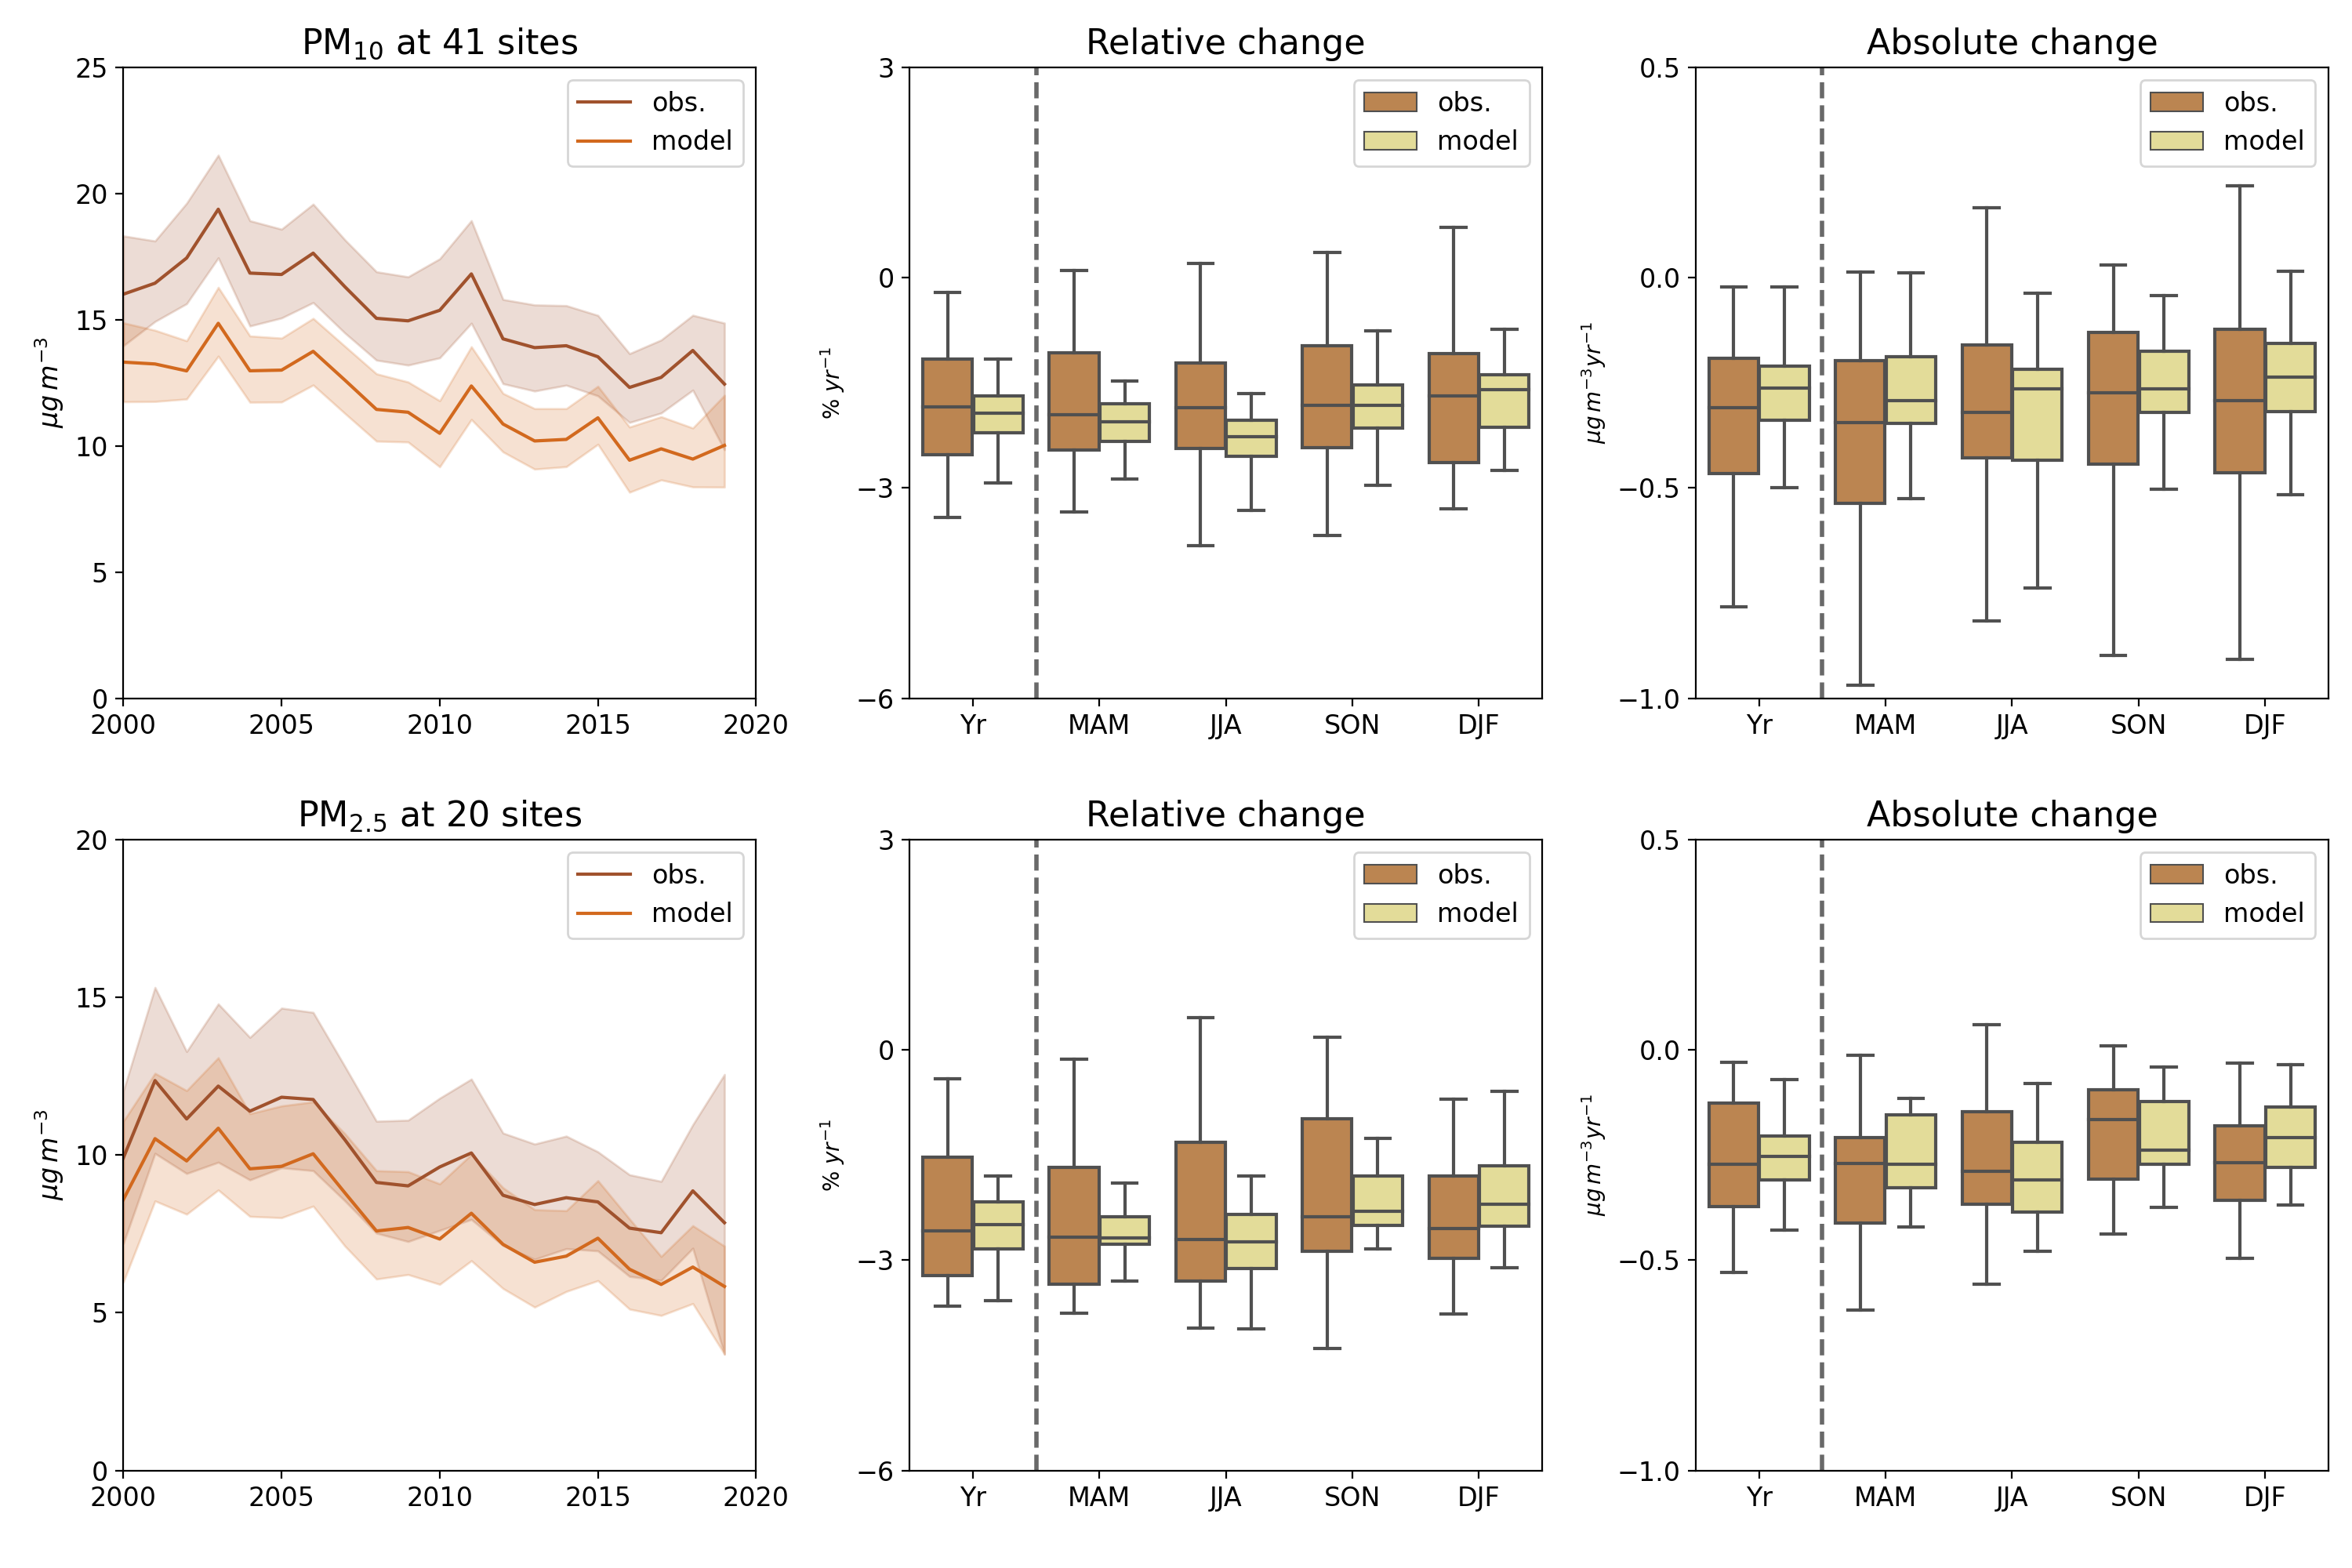
\includegraphics[width=0.74\paperwidth]{FIGS_TRENDS/PM_trends.png}
	\caption{\label{fig:pm_trends}Trends in \PM[10]  and \PM[2.5] from 2010-2019 for EMEP observations and model: left panels - annual timeseries (the solid line indicates the average annual mean trend for all sites, the shaded area shows the 95 \% confidence interval); middle and right panels - relative and absolute trends for all the sites, with both significant and not significant trends (the boxes represent the 50,25,75 percentiles, the whiskers lie within the 1.5 inter-quartile ranges, the mean trends are indicated with black circles}
\end{figure}


\begin{table}
\caption{\label{tab:pm10_stat} Average absolute and relative changes in \PM[10]}
\begin{center}
\scalebox{0.65}{%
\begin{tabular}{ll|ccc|cccc|cccc}
\toprule
          &        & \multicolumn{3}{c}{Number of sites} & \multicolumn{4}{c}{Average change per year (\ug $yr^{-1})$} & \multicolumn{4}{c}{Relative change per year (\% $yr^{-1}$)} \\
Period & Seasons &           total & sign.(obs.) & sign.(mod.) &                    obs. &          conf.interval &  mod. &          conf.interval &                     obs. &         conf.interval &  mod. &        conf.interval \\
\midrule
2000-2019 & all &              37 &          29 &          36 &                   -0.36 &  (-0.43, -0.29) & -0.27 &  (-0.31, -0.24) &                    -1.83 &  (-2.09, -1.57) & -1.92 &  (-2.08, -1.75) \\
          & autumn &              35 &          22 &          29 &                   -0.34 &  (-0.42, -0.26) & -0.27 &  (-0.31, -0.24) &                    -1.81 &   (-2.1, -1.51) & -1.85 &  (-2.03, -1.67) \\
          & spring &              34 &          24 &          32 &                   -0.39 &  (-0.47, -0.31) & -0.29 &  (-0.34, -0.25) &                    -1.84 &  (-2.11, -1.56) & -2.04 &  (-2.23, -1.86) \\
          & summer &              36 &          27 &          32 &                   -0.34 &  (-0.42, -0.25) & -0.30 &  (-0.35, -0.24) &                    -1.72 &  (-2.09, -1.35) & -2.22 &  (-2.44, -1.99) \\
          & winter &              34 &          18 &          20 &                   -0.36 &  (-0.47, -0.25) & -0.27 &  (-0.32, -0.22) &                    -1.73 &   (-2.07, -1.4) & -1.69 &   (-1.88, -1.5) \\
2005-2019 & all &              54 &          29 &          37 &                   -0.33 &  (-0.41, -0.25) & -0.22 &  (-0.26, -0.19) &                    -1.82 &  (-2.23, -1.41) & -1.80 &  (-2.05, -1.54) \\
2010-2019 & all &              56 &          17 &          26 &                   -0.32 &  (-0.42, -0.21) & -0.17 &  (-0.22, -0.13) &                    -1.84 &  (-2.45, -1.23) & -1.51 &   (-1.9, -1.12) \\
2000-2010 & all &              36 &          14 &          23 &                   -0.46 &  (-0.56, -0.36) & -0.32 &  (-0.42, -0.22) &                    -2.36 &  (-2.77, -1.95) & -2.25 &  (-2.83, -1.68) \\
\bottomrule
\end{tabular}}
\end{center}
\end{table}

\begin{table}
\caption{\label{tab:pm25_stat} Average absolute and relative changes in \PM[25]}
\begin{center}
\scalebox{0.65}{%
\begin{tabular}{ll|ccc|cccc|cccc}
\toprule
          &        & \multicolumn{3}{c}{Number of sites} & \multicolumn{4}{c}{Average change per year (\ug $yr^{-1})$} & \multicolumn{4}{c}{Relative change per year (\% $yr^{-1}$)} \\
Period & Seasons &           total & sign.(obs.) & sign.(mod.) &                    obs. &          conf.interval &  mod. &          conf.interval &                     obs. &         conf.interval &  mod. &        conf.interval \\
\midrule
2000-2019 & all &              19 &          16 &          19 &                   -0.29 &   (-0.39, -0.2) & -0.25 &  (-0.29, -0.21) &                    -2.42 &   (-2.84, -2.0) & -2.50 &  (-2.71, -2.29) \\
          & winter &              18 &          12 &          14 &                   -0.36 &  (-0.54, -0.18) & -0.21 &  (-0.25, -0.17) &                    -2.29 &  (-2.74, -1.85) & -2.11 &  (-2.39, -1.83) \\
          & spring &              19 &          14 &          19 &                   -0.32 &  (-0.41, -0.24) & -0.26 &   (-0.3, -0.22) &                    -2.47 &  (-2.91, -2.03) & -2.64 &  (-2.82, -2.45) \\
          & summer &              18 &          14 &          17 &                   -0.26 &  (-0.33, -0.19) & -0.28 &  (-0.35, -0.22) &                    -2.36 &  (-2.91, -1.82) & -2.78 &  (-3.12, -2.45) \\
          & autumn &              18 &          12 &          16 &                   -0.26 &  (-0.36, -0.15) & -0.24 &  (-0.31, -0.17) &                    -2.22 &  (-2.71, -1.74) & -2.24 &  (-2.47, -2.01) \\
2005-2019 & all &              36 &          23 &          27 &                   -0.33 &  (-0.42, -0.23) & -0.21 &  (-0.25, -0.17) &                    -2.66 &  (-3.16, -2.16) & -2.28 &  (-2.53, -2.04) \\
2010-2019 & all &              43 &          20 &          19 &                   -0.34 &  (-0.43, -0.25) & -0.19 &  (-0.24, -0.14) &                    -3.14 &   (-3.7, -2.57) & -2.28 &  (-2.71, -1.85) \\
2000-2010 & all &              20 &           7 &          13 &                   -0.36 &   (-0.5, -0.21) & -0.34 &  (-0.43, -0.25) &                    -2.65 &  (-3.56, -1.73) & -2.88 &  (-3.51, -2.25) \\
\bottomrule
\end{tabular}}
\end{center}
\end{table}


For the whole period, 36 and 18 sites with satisfactory data coverage have been included in the trend analysis respectively for \PM[10] and \PM[2.5]. The annual series of \PM[10] and \PM[2.5] clearly show a general concentration decrease from 2000 to 2019. In general, the model reproduces quite well observed year-to-year changes in \PM[10] and \PM[2.5], including enhanced PM levels due to meteorological conditions e.g. in 2003 (dry hot summer \citep{EMEP:PM2005}) and 2011 (dry year in Western/Central/Southern Europe \citep{EMEP:PM2013}).

Summarizing overall results, the average \PM[10] and \PM[2.5] trends, derived from observational data and model simulations, are decreasing for the 2000-2019 period (and for all considered here periods). In relative terms, \PM[2.5] average decreasing trend was larger than that for \PM[10]. The PM trends can be explained by decreases in the concentrations of the individual components due to emission reductions, with \PM[10] trends experiencing larger disturbances due to natural contribution in the coarse fraction. We find a good correspondence between observed and model simulated trends in PM concentrations at the considered sites. A more detailed discussion of PM trends follows below.
In the period of 2000-2019, the average observed \PM[10] trends are -0.37 \ug $yr^{-1}$, or -1.86 \% $yr^{-1}$ in relative terms. The corresponding \PM[10] trends from model simulations are -0.28 \ug $yr^{-1}$ and -1.91 \% $yr^{-1}$. For \PM[2.5], the average trends are -0.31 and -0.25 \ug $yr^{-1}$ respectively from the observations and model simulations, and the relative decrease of \PM[2.5] is -2.51 \% $yr^{-1}$, both observed and modelled. 


Significant trends have been derived from the observational data for 80 \% of sites for \PM[10] and 97 \% of sites for \PM[2.5]; the model simulates significant trends for more sites, namely 97 and 100 \% respectively.  

Figure \ref{fig:pm_trends} reveals a considerably larger variation of observed trends between the sites in comparison to modelled trend values, \textcolor{blue}{with modelled median (and mean) trends lying within 25-75\% interquartile range (IQR) of the observed ones. Modelled mean and median trends are in general closer to each other than in the observational data, implying more sites-outliers.} The model simulated the largest \PM[10] and \PM[2.5] 2000-2019 trends, both absolute and relative,  for the summer season, followed by the spring, whereas the observation results are less conclusive in this respect. However, both the observations and the model identify PM significant trends for more stations for the spring and summer seasons than for the winter-autumn. 

Thus, for the period 2000-2019, the observations show a decrease of \PM[10] and \PM[2.5] concentrations by 36 and 48 \% respectively, which is in a perfect agreement with modelled decreases by 36 and 48 \% respectively. PM is a complex pollutant, consisting of aerosol species both emitted directly and formed from gaseous precursors. Therefore, the reductions both in primary PM emissions, as well as \sox, \noii, \nhiii and NMVOC emissions are contribute to decrease PM concentrations. In the western parts of EMEP (EU \&UK \&EFTA), where the considered sites are located, the emissions of primary \PM[10] and \PM[2.5] were reduced by 32 and 35 \%, respectively, from 2000 to 2019. The largest in the same period, was reduction in \sox emissions (81 \%), resulting in 61 \% observed decrease of \soiv (70 \% according to the model). Though \noii was reduced by 48 \%, given the moderate reduction by 12 \% in \nhiii emissions and the availability of free \nhiii due to the reduced formation of ammonium sulphate, the observed decrease in \noiii concentrations was only 38 \% (44 \% by the model). The corresponding changes from 2000 to 2019 in \nhiv were 50 and 48 \%.

For the period 2005-2019 (starting from the reference year of Gothenburg Protocol), more sites with data coverage were totally available for this \PM[10] and \PM[2.5] trend analysis, i.e. 53 and 35 respectively, but significant trends have been observed and modelled for a smaller fraction of the sites with respect to the 2000-2019 period \textcolor{blue}{(partly due to a shorter period length)}.




\section{\label{sec:Trends_O3 }Trends in O$_3$ }



\begin{figure}
	\centering
	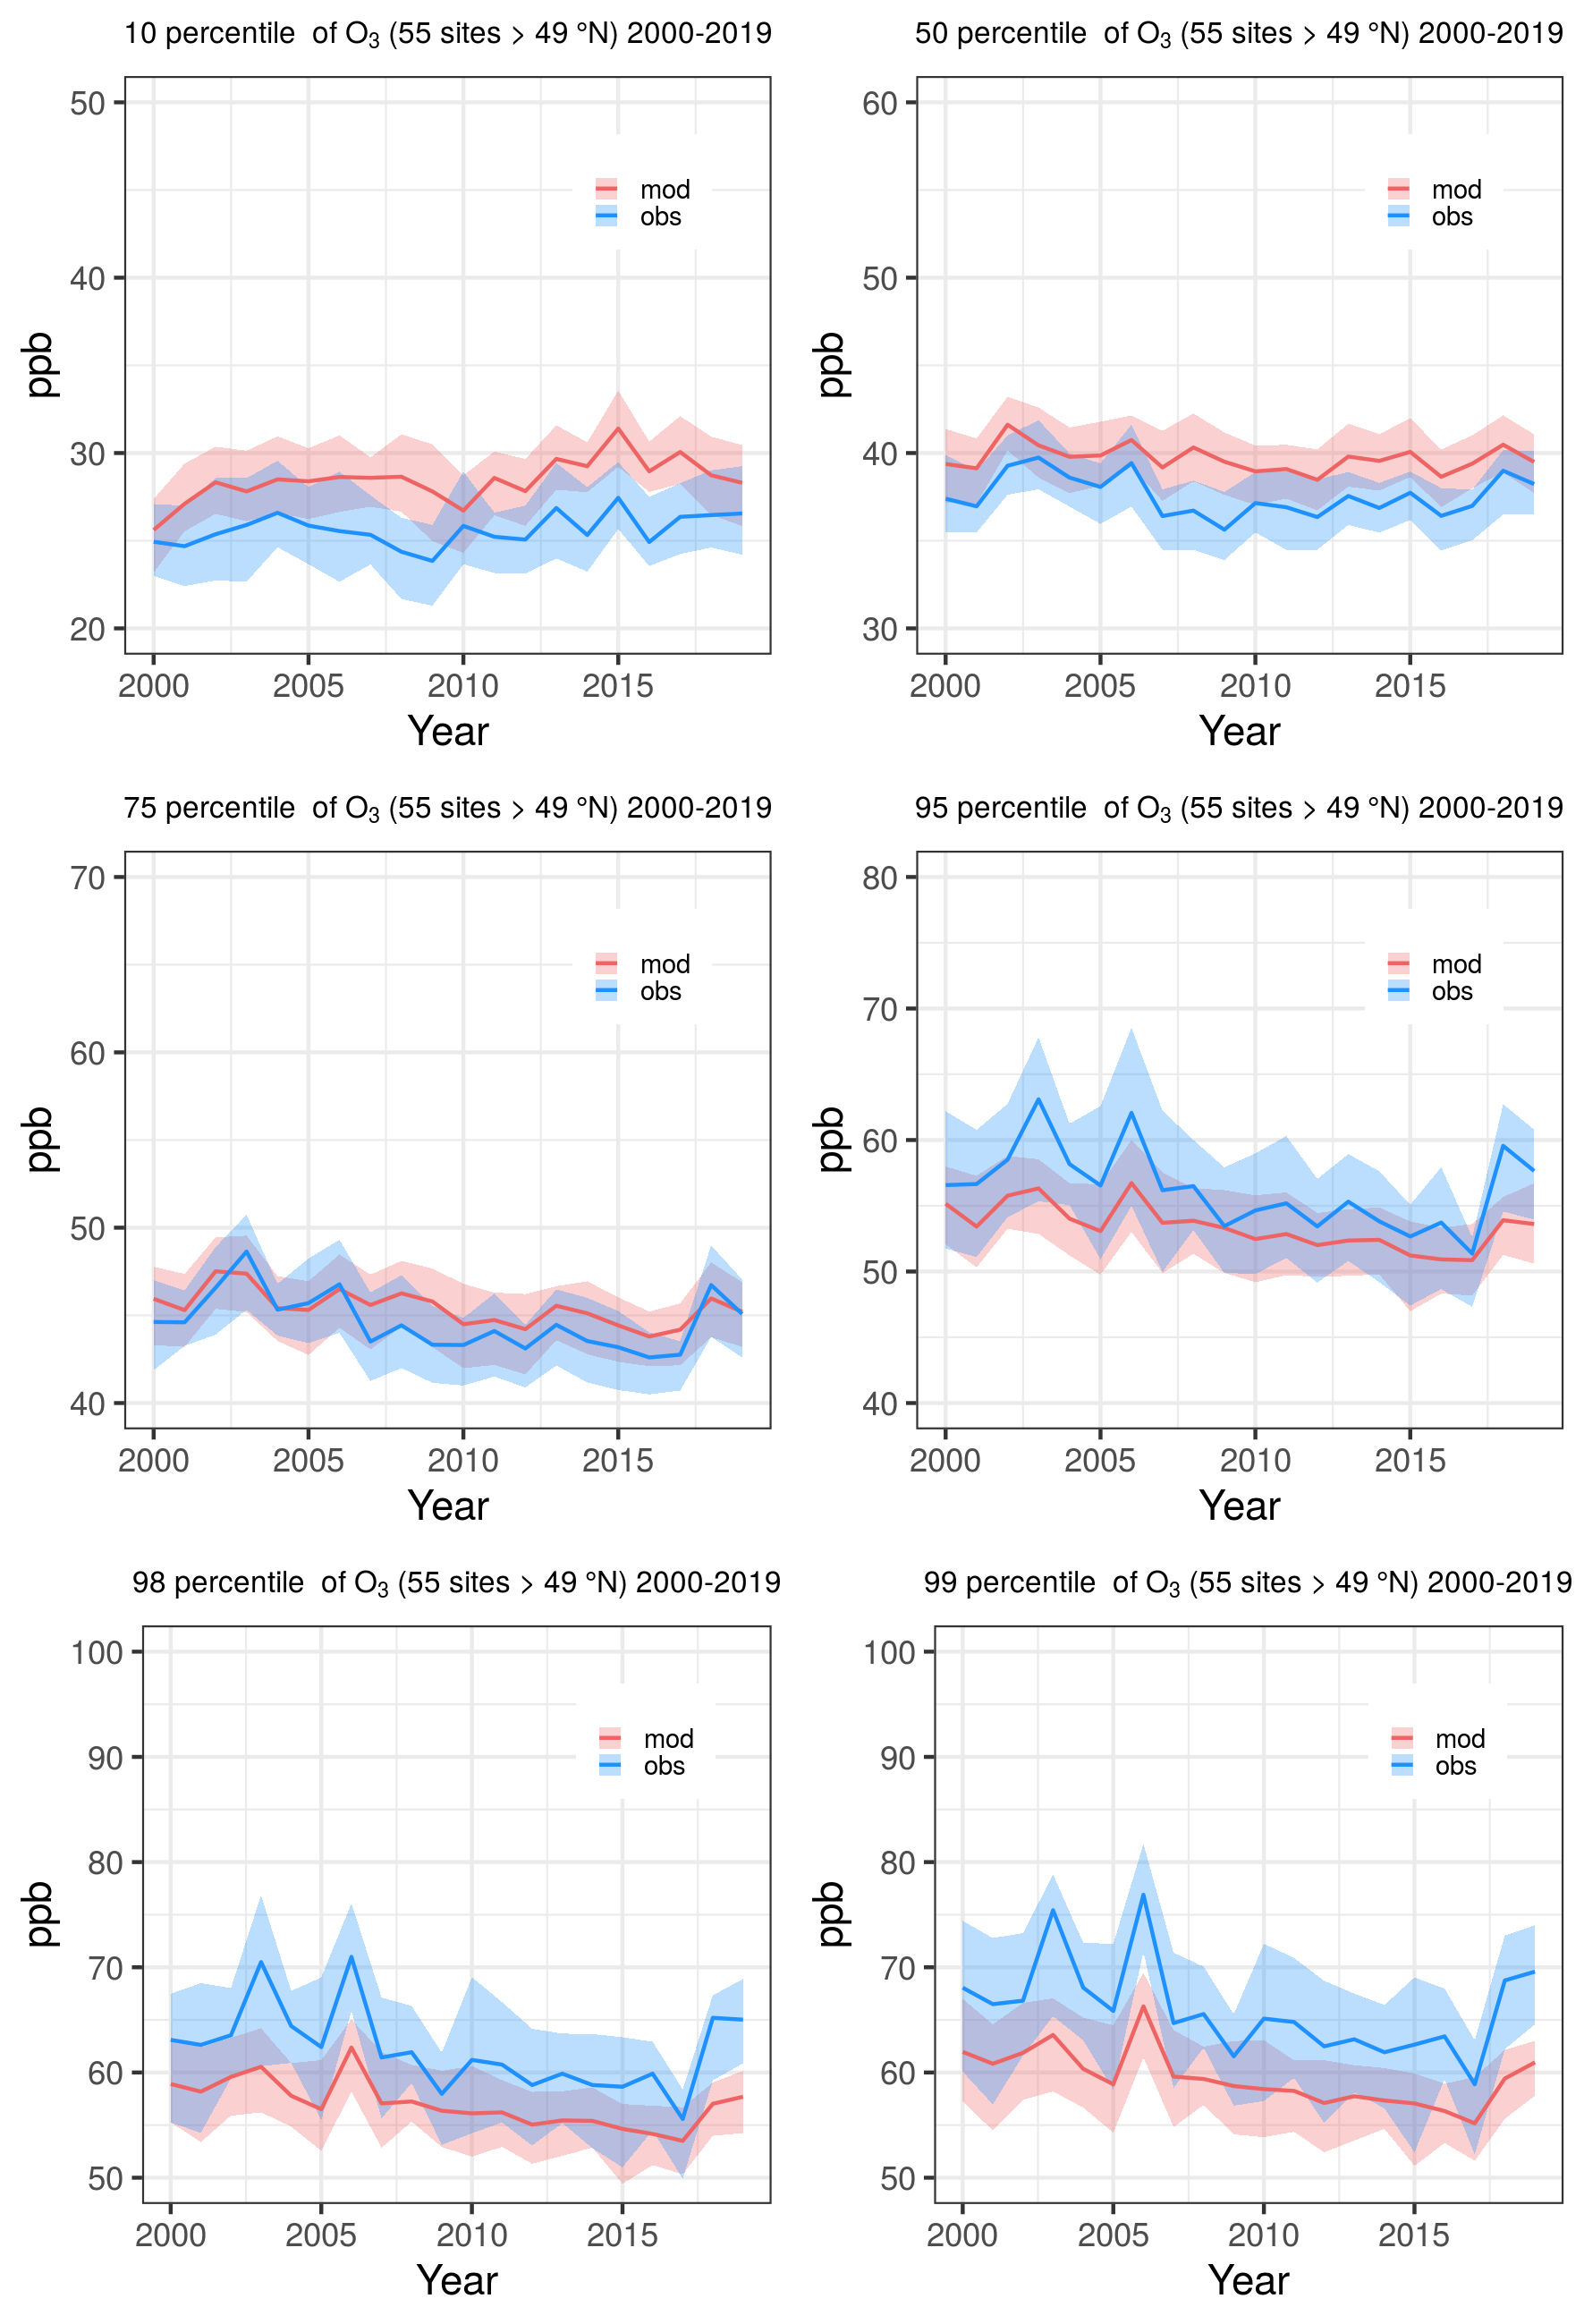
\includegraphics[width=0.74\paperwidth]{FIGS_TRENDS/alltrends_north_49_2000_2019_1200m.png}
	\caption{\label{fig:O3_perctrends_N}Trends in annual percentiles of daily max O$_3$ from 2000-2019 for EMEP observations and model for sites north of 49 N: The solid line indicates the mean, and the shaded area marks the 25 and 75 percentile. Only sites below 1200 m asl and with at least 15 years of data are included.}
\end{figure}

\begin{figure}
	\centering
	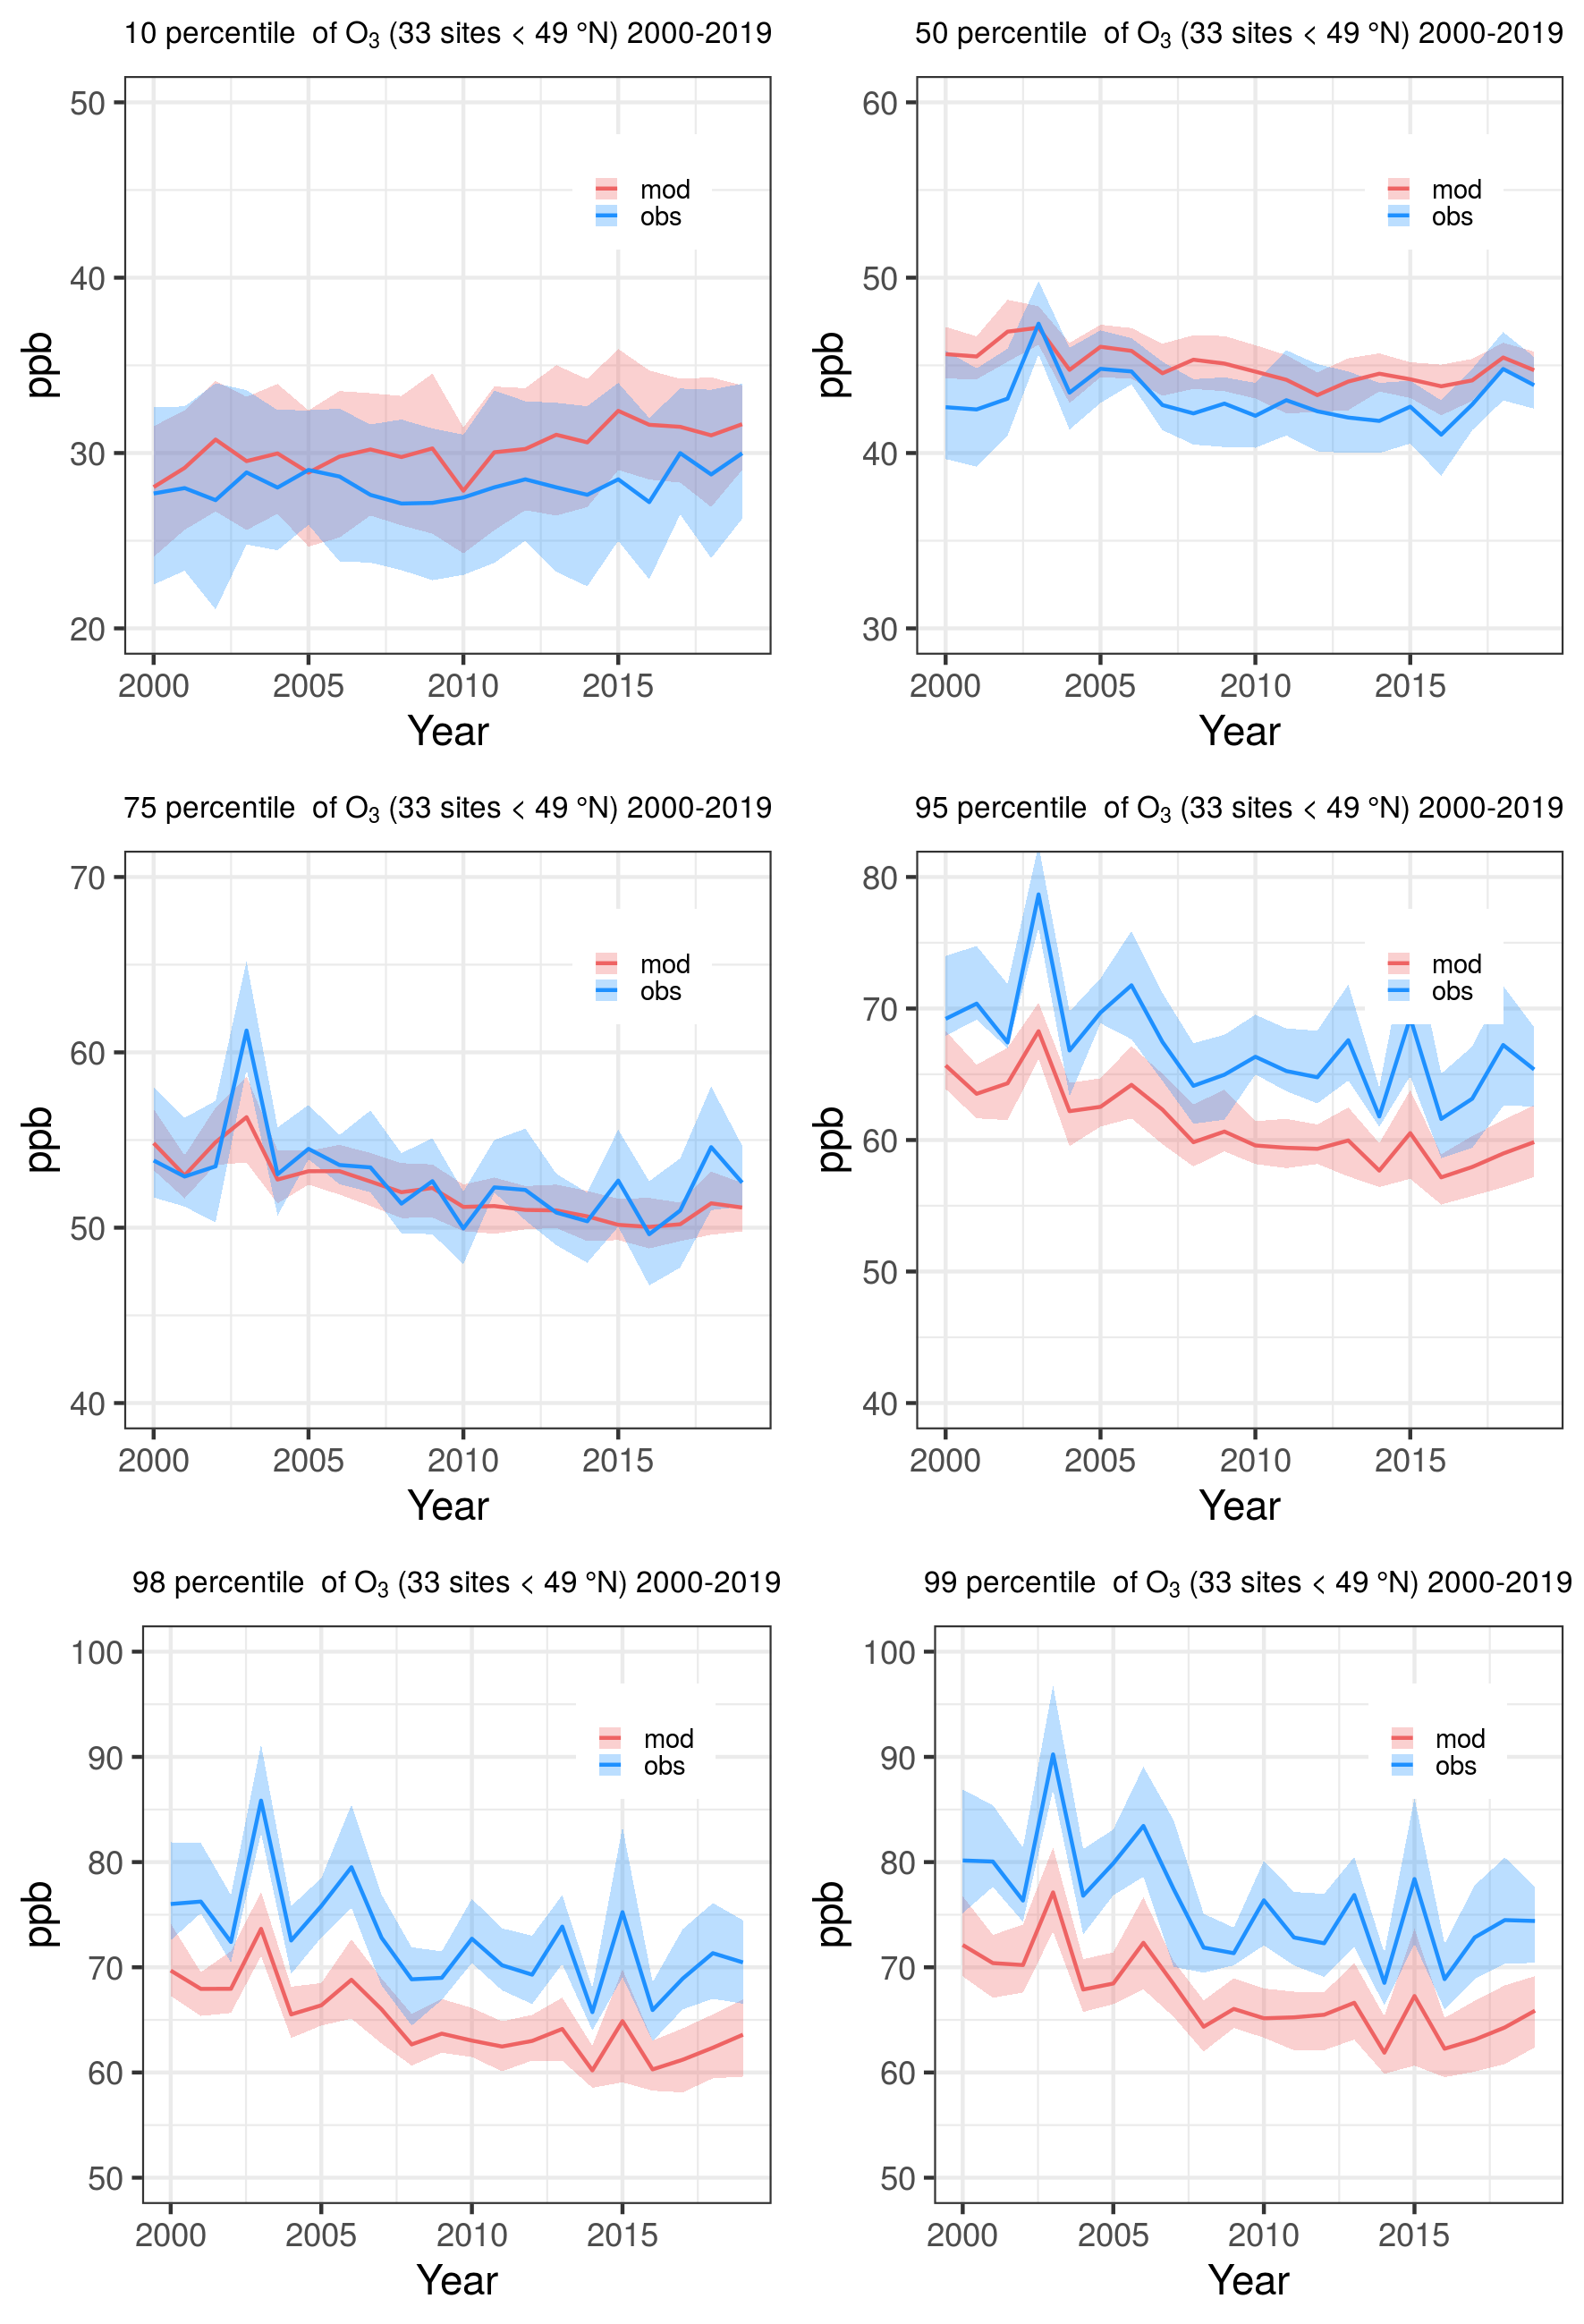
\includegraphics[width=0.74\paperwidth]{FIGS_TRENDS/alltrends_south_49_2000_2019_1200m.png}
	\caption{\label{fig:O3_perctrends_S}Trends in annual percentiles of daily max O$_3$ from 2000-2019 for EMEP observations and model for sites south of 49 N: The solid line indicates the mean, and the shaded area marks the 25 and 75 percentile. Only sites below 1200 m asl and with at least 15 years of data are included.}
\end{figure}


\begin{figure}
	\centering
	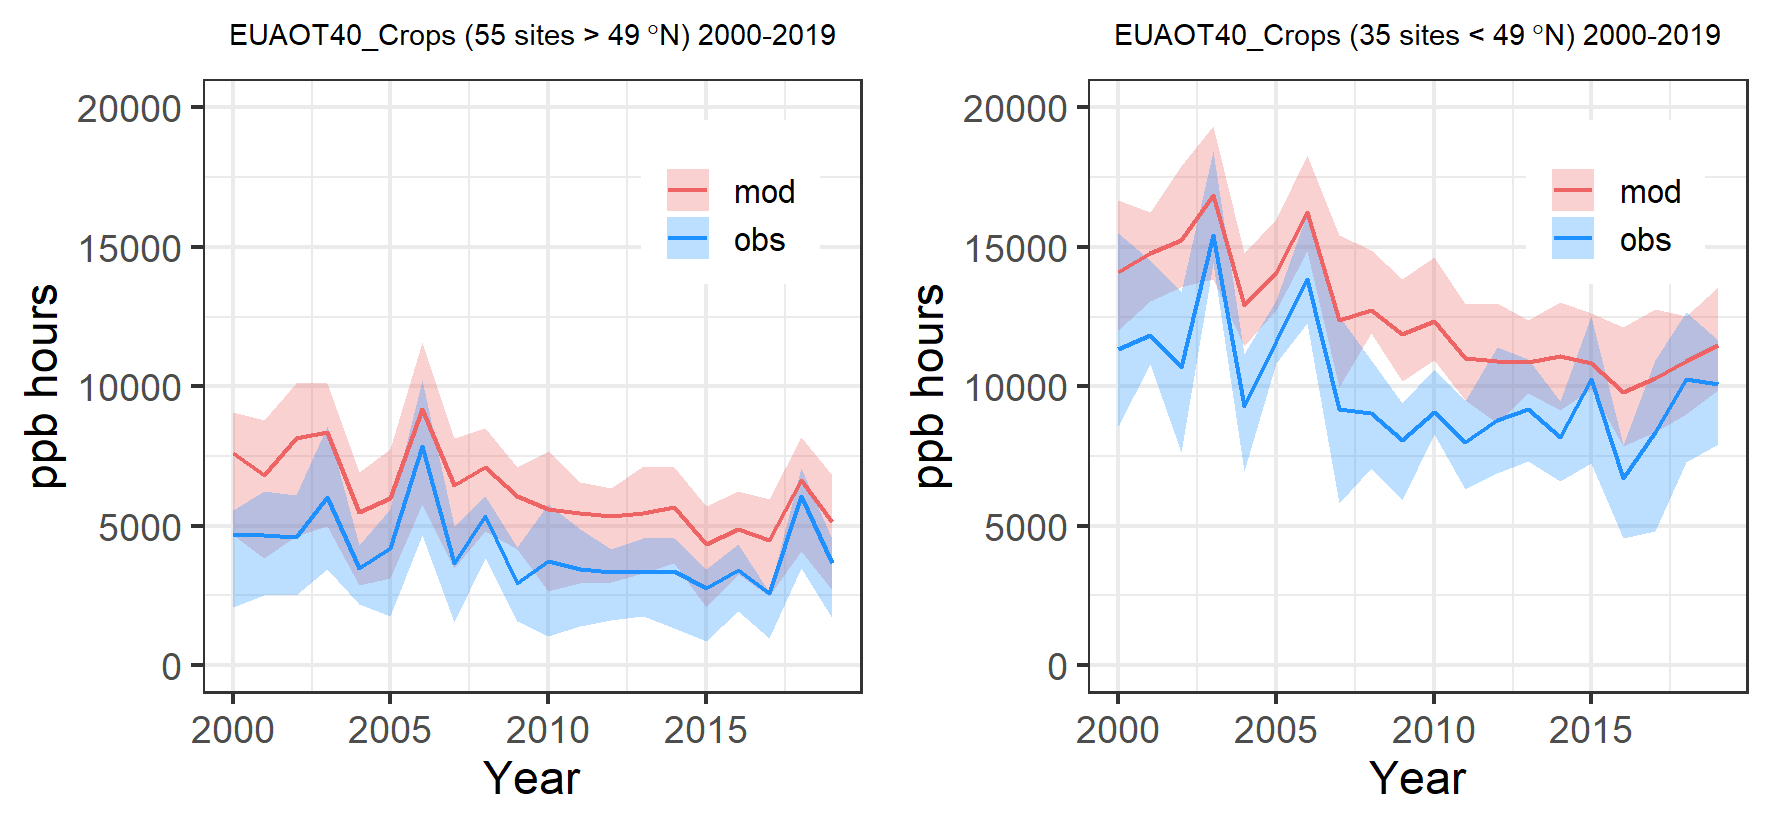
\includegraphics[width=0.74\paperwidth]{FIGS_TRENDS/EUAOT40_Crops_2000_2019_1200m.png}
	\caption{\label{fig:O3_aot40croptrends} Trends in 3-months AOT40 (May-July) O$_3$ for crops from 2000-2019 for EMEP observations and model for sites north (left) and south (right) of 49 N: The solid line indicates the mean, and the shaded area marks the 25 and 75 percentile. Only sites below 1200 m asl and with at least 15 years of data are included.}
\end{figure}

\begin{figure}
	\centering
	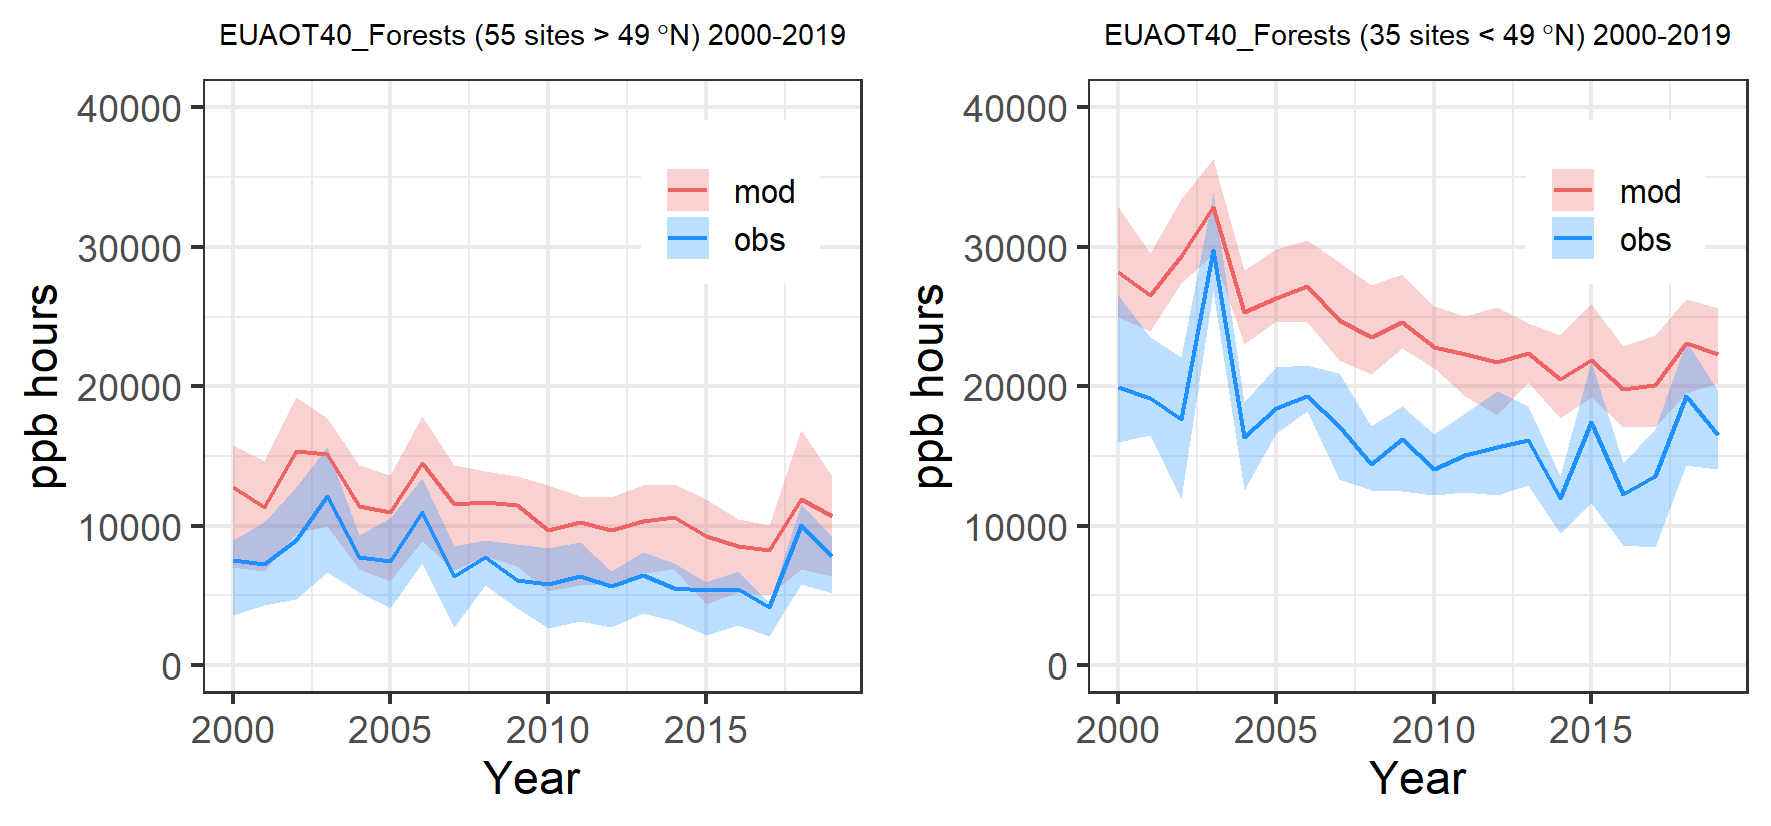
\includegraphics[width=0.74\paperwidth]{FIGS_TRENDS/EUAOT40_Forests_2000_2019_1200m.png}
	\caption{\label{fig:O3_aot40foresttrends}Trends in 6-months AOT40 (Apr-Sep) O$_3$ for forests from 2000-2019 for EMEP observations and model for sites north (left) and south (right) of 49 N: The solid line indicates the mean, and the shaded area marks the 25 and 75 percentile. Only sites below 1200 m asl and with at least 15 years of data are included.}
\end{figure}

\begin{figure}
	\centering
	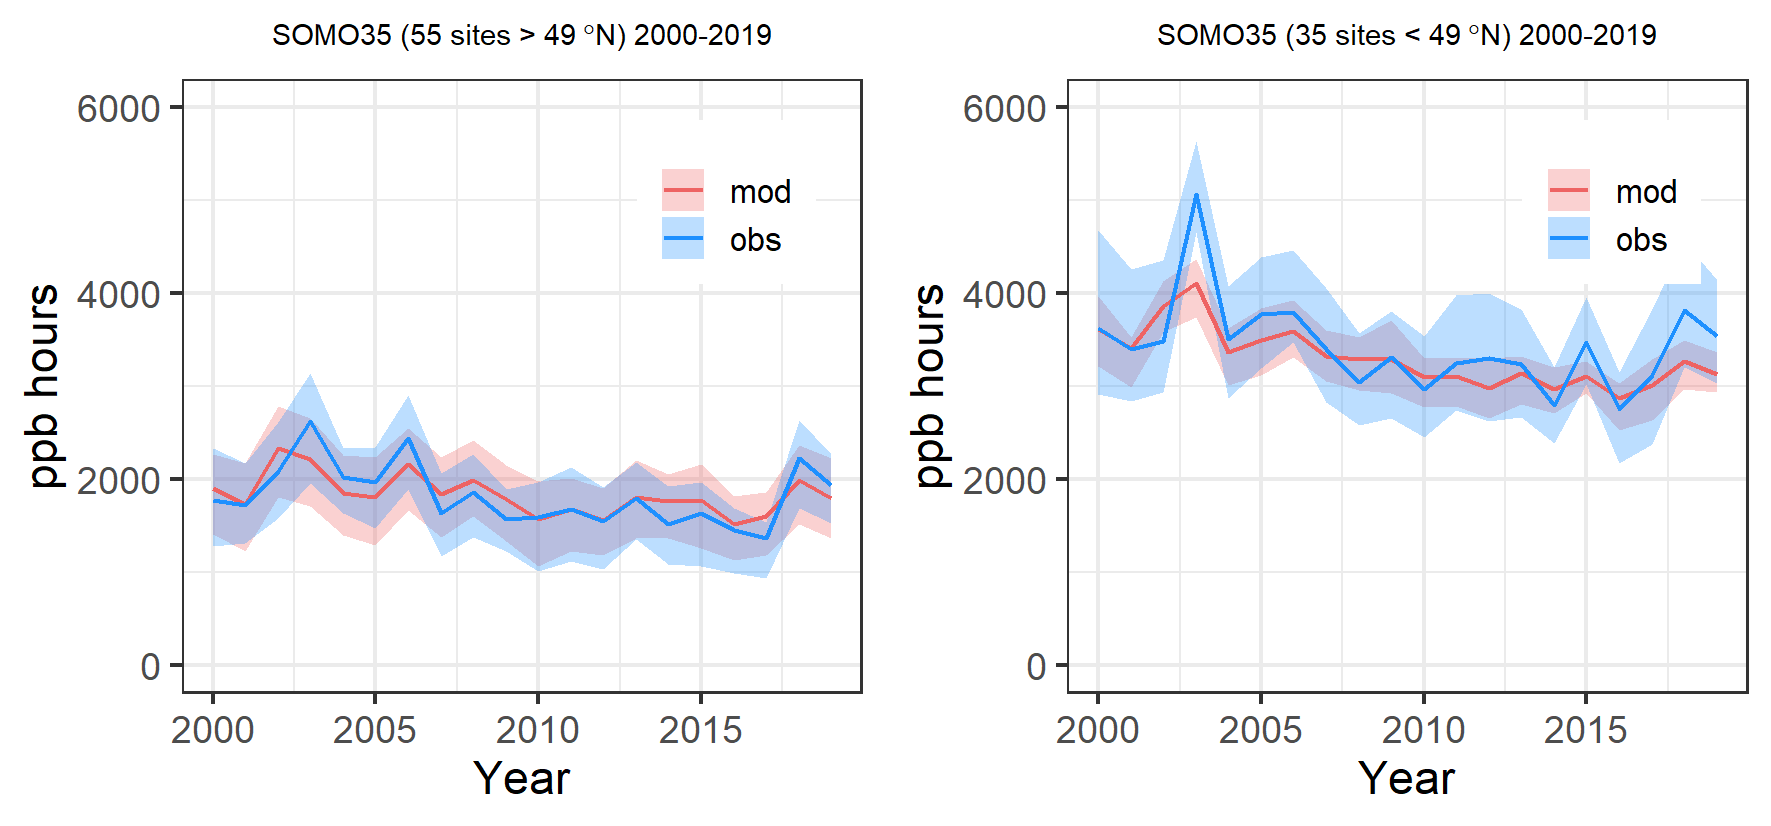
\includegraphics[width=0.74\paperwidth]{FIGS_TRENDS/SOMO35_2000_2019_1200m.png}
	\caption{\label{fig:O3_somo35trends}Trends in SOMO35 from 2000-2019 for EMEP observations and model for sites north (left) and south (right) of 49 N: The solid line indicates the mean, and the shaded area marks the 25 and 75 percentile. Only sites below 1200 m asl and with at least 15 years of data are included.}
\end{figure}

\section{Exceedances of critical loads of acidification and eutrophication in 2000 to 2019.}
\label{subs:exceedSnN}
%Thomas/CCE: I just updated this section. Please have a look TS 17.08.2021

The exceedances of European critical loads (CLs) are computed for the total nitrogen
(N) and sulphur (S) depositions modelled on the 0.1$\degrees \times$ 0.1$\degrees$
longitude-latitude grid (approx. 11 x 5.5 km$^{2}$ at 60$\degrees$N).
Exceedances are calculated for the European critical loads documented in \cite{Hettelingh:2017}, while
a description of the methods is given in \cite{DeVries:2015}. The
critical loads data for eutrophication by N (CL eut N) and for acidification by N and S
(CL acid) are also used by the EMEP Centre CIAM (located at IIASA) in their integrated assessment
modelling. The exceedance in a grid cell is the so-called ’average accumulated
exceedance’ (AAE), which is calculated as the area-weighted average of the
exceedances of the critical loads of all ecosystems in this grid cell. The units for
critical loads and their exceedances are equivalents (eq; same as \textit{moles of charge},
molc) per area and time, making S and N depositions comparable on their impacts, which is important for
acidity CLs.

Critical loads are available for about 4 million ecosystems in Europe covering an area
of about 3 million km$^{2}$ (west of 42$\degrees$E). The exceedances (AAE) of those critical loads
are computed on a 0.1$\degrees \times$ 0.1$\degrees$ longitude-latitude grid, and maps for the deposition in
the years 2000, 2005, 2010, 2015 and 2019 are shown in Figures \ref{fig:eutN} and \ref{fig:acid}. As indicated in the maps, the critical loads for eutrophication are exceeded in practically all countries in all years. The share of ecosystems where the critical load for eutrophication is exceeded decreases relatively slowly, starting at 76.4\% in 2000 and ending at 65.5\% in 2019.
European average AAE is about 452 eq ha$^{-1}$ yr$^{-1}$ (2000) and 276 eq
ha$^{-1}$ yr$^{-1}$ (2019). The highest exceedances of CLs are found in the Po Valley in Italy, the
Dutch-German-Danish border areas and in north-eastern Spain.
By contrast, critical loads of acidity are exceeded in a much smaller area. Hot spots of
exceedances can be found in the Netherlands and its border areas to Germany and
Belgium, and some smaller maxima in southern Germany and Czechia,
whereas most of Europe is not exceeded (grey areas). Acidity exceedances occur
on 16.2\% (2000) and 5.0\% (2019) of the ecosystem area and the European average
AAE is about 133 eq ha$^{-1}$ yr$^{-1}$ (2000) and 25 eq ha$^{-1}$ yr$^{-1}$ (2019). Overall statistics for the share of critical load exceedance and European average of AAE are shown in Figures \ref{fig:stats_cl_ex}.
\begin{figure}[ht]
  \centering
  \subfigure{\includegraphics*[scale=0.20]{FIGS_CL_Exceedance/Stats_CLex_eut.png}}
  \subfigure{\includegraphics*[scale=0.20]{FIGS_CL_Exceedance/Stats_CLex_acid.png}}
  \caption{Summary for exceedance of critical load for eutrophication (left) and acidification (right).}
\label{fig:stats_cl_ex}
\end{figure}
\begin{figure}[ht]
  \centering
  \subfigure{\includegraphics*[scale=0.35]{FIGS_CL_Exceedance/CL_Ex_eut_2000.png}}
  \subfigure{\includegraphics*[scale=0.35]{FIGS_CL_Exceedance/CL_Ex_eut_2005.png}}
  \subfigure{\includegraphics*[scale=0.35]{FIGS_CL_Exceedance/CL_Ex_eut_2010.png}}
  \subfigure{\includegraphics*[scale=0.35]{FIGS_CL_Exceedance/CL_Ex_eut_2015.png}}
  \subfigure{\includegraphics*[scale=0.35]{FIGS_CL_Exceedance/CL_Ex_eut_2019.png}}
 \caption{Exceedance of critical load for eutrophication for the years 2000, 2005, 2010, 2015 and 2019.}
\label{fig:eutN}
\end{figure}
\begin{figure}[ht]
  \centering
 \subfigure{\includegraphics*[scale=0.35]{FIGS_CL_Exceedance/CL_Ex_acid_2000.png}}
  \subfigure{\includegraphics*[scale=0.35]{FIGS_CL_Exceedance/CL_Ex_acid_2005.png}}
  \subfigure{\includegraphics*[scale=0.35]{FIGS_CL_Exceedance/CL_Ex_acid_2010.png}}
  \subfigure{\includegraphics*[scale=0.35]{FIGS_CL_Exceedance/CL_Ex_acid_2015.png}}
  \subfigure{\includegraphics*[scale=0.35]{FIGS_CL_Exceedance/CL_Ex_acid_2019.png}}
 \caption{Exceedance of critical load for acidification for the years 2000, 2005, 2010, 2015 and 2019.}
\label{fig:acid}
\end{figure}





%DAVE MOVED TO END OF chapterTrendsECOC.tex

